
% !TeX spellcheck = en_US
 %!TeX spellcheck = el_EL-ModernGreek
\documentclass[12pt,a4paper]{article}
\usepackage[utf8]{inputenc}
\usepackage[T1]{fontenc}
\usepackage{amsmath}
\usepackage{amssymb}
\usepackage{graphicx}
\usepackage{fancyhdr}
\usepackage[left=1.50cm, right=1.50cm, top=1.50cm, bottom=1.50cm, includeheadfoot]{geometry}
\usepackage[greek]{babel}
\usepackage{fontspec}
\setmainfont{Verdana}
\usepackage[hidelinks]{hyperref}
\usepackage{subfigure}
\usepackage{dirtree}
\usepackage{float}
\usepackage{wrapfig}
\usepackage{color}


\pagestyle{fancy}
\lhead{LAB3 Report}
\rhead{Υλοποίηση VGA controller}
\setlength{\headheight}{15pt}

\title{\textbf{\textcolor{red}{\underline{LAB3: Υλοποίηση Ελεγκτή VGA driver}} } }
\author{Δημήτριος Τσαλαπάτας, ΑΕΜ: 03246}
\date{18 Δεκεμβρίου 2022}

\begin{document}
	\maketitle
	\tableofcontents
	\newpage
	\section{\textcolor{cyan}{Περίληψη} }
	Για την υλοποίηση του VGA controller χρειάστηκε να δημιουργήσουμε τέσσερα modules. Αρχικά, υλοποιούμε την VRAM για να διαβάζει το vga την εικόνα, στην συνέχεια τα σήματα συγχρονισμού HSYNC και VSYNC, και τέλος το top module όπου αποτελεί την σύνδεση όλων αυτών και την υλοποίηση του VGA controller. Μετά από ελέγχους και πειραματικές διεργασίες, υλοποιούμε ένα λειτουργικό VGA controller για συμβατικές οθόνες τύπου CRT. Εκτενής ανάλυση για το κύκλωμα ακολουθεί παρακάτω.
	
	\section{\textcolor{cyan}{Εισαγωγή} }
	Η τρίτη εργαστηριακή άσκηση έχει σαν στόχο την υλοποίηση ενός οδηγού θύρας οθόνης VGA ώστε να μπορεί να απεικονίσει μία προεπιλεγμένη σταθερή εικόνα της επιλογής μας σε μία συμβατική οθόνη. Πιο συγκεκριμένα, απαιτείται να απεικονίζεται μία εικόνα με διάφορα χρώματα και μοτίβο σε ανάλυση 640x480 pixels και ρυθμό ανανέωσης οθόνης τα 60Hz.\\
	Αρχικά, είναι απαραίτητο να χρησιμοποιηθεί ένα κομμάτι από τις μνήμες της FPGA για να αποθηκευτεί η εικόνα που θέλουμε να απεικονίσουμε \emph{VRAM} το οποίο επιτεύχθηκε με την δημιουργία ενός module που περιλαμβάνει μία μνήμη για κάθε χρώμα που θέλουμε να αποτυπώσουμε. Στην συνέχεια, ήταν αναγκαίος ο συγχρονισμός των δύο βασικών σημάτων για την λειτουργία του VGA, των \emph{HSYNC} και \emph{VSYNC} για οριζόντιο και κατακόρυφο συγχρονισμό αντίστοιχα, το οποίο επιτεύχθηκε με την υλοποίηση μίας FSM για καθένα με τις κατάλληλες καταστάσεις και κυρίως με τους \underline{κατάλληλους χρόνους}.

	
	\section{\textcolor{cyan}{Μέρος Α - Υλοποίηση VRAM}}
	\subsection{\textcolor{black}{VRAM modules} }
	Για να είναι δυνατή η προβολή μίας σταθερής εικόνας στην οθόνη θα πρέπει να βρίσκεται κάπου μέσα στις μνήμες της FPGA ώστε να έχει την δυνατότητα το VGA να πάρει την κατάλληλη πληροφορία για να ζωγραφίσει την εικόνα στην οθόνη.//
	Αρχικά, τα χρώματα που χρησιμοποιούνται για την απεικόνιση οποιουδήποτε χρώματος στο VGA είναι τα red (r), green (g) και blue (b), οπότε από τον συνδιασμό των RGΒ προκύπτουν τα υπόλοιπα χρώματα που επιθυμούμε. Το σκεπτικό είναι ότι για κάθε pixel της εικόνας αποθηκεύουμε τις τιμές των RGB στην μνήμη για να απεικονιστεί το χρώμα που θέλουμε. Για την περίπτωση της εργασίας κάθε χρώμα είναι μεγέθους 1bit δηλαδή απλά αν είναι αναμμένο ή σβηστό το χρώμα (σε αντίθεση με το κανονικό VGA που οι τιμές ποικίλουν από 3-4 bit ανά χρώμα). Οπότε οι συνδυασμοί χρωμάτων που προκύπτουν είναι οι παρακάτω:
	\begin{figure} [htbp]
		\centering{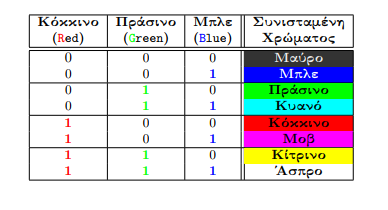
\includegraphics[width=0.5\textwidth]{pictures/colors} }
		\caption{Colours combinations}
		\label{Colours combinations}
	\end{figure}
	
	Οπότε εφόσον η εικόνα μας θα πρέπει να είναι ανάλυσης 640x480 pixels, χρειαζόμαστε μνήμη ίση με $640*480 = 307.200 bits$ για το ένα χρώμα άρα για τα 3 $921.600 bits$. Η FPGA όμως δεν περιέχει τόσο μεγάλη συνεχόμενη μνήμη καθώς βρίσκεται σε blocks, οπότε θα αποτυπώσουμε μία εικόνα ανάλυσης 128x96 και θα γίνει upscale από τον συγχρονισμό το οποίο θα αναλυθεί παρακάτω. Για να χρησιμοποιήσουμε σωστά την μνήμη θα χρησιμοποιήσουμε ένα template απο το vivado το \verb*|BRAM_SINGLE_MACRO| το οποίο προσφέρει διάφορες επιλογές για το μέγεθος της μνήμης καθώς επίσης και του μεγέθους των bits που θα διαβάζονται ή γράφονται. Επιλέγουμε τον συνδυασμό 1*18kb, οπότε προκύπτει από το manual ότι έχουμε διαθέσιμα για διάβασμα 16.384 bits (αρκετά για τις ανάγκες μας). Θα χρησιμοποιήσουμε τρία blocks της μνήμης, μία για κάθε χρώμα, και θα αρχικοποιήσουμε ανάλογα κάθε block για κάθε χρώμα ώστε να αποτυπωθεί η εικόνα που επιθυμούμε. Προσοχή χρειάζεται ότι η μνήμη διαβάζει από δεξιά προς τα αριστερά, ενώ έτσι όπως είναι χωρισμένες οι γραμμές, κάθε γραμμή στο instantiation της μνήμης αποτελεί δύο γραμμές για την οθόνη, καθώς είναι 256 bits ενώ η οθόνη 128.\\
	Η εικόνα που επιλέχθηκε να εκτυπώσουμε στην οθόνη αποτελείται από ένα μοτίβο εναλλαγής μεταξύ κόκκινου, άσπρου, πράσινου και γαλάζιου και στην συνέχεια δύο κάθετες στήλες πράσινου και μπλε.
	\begin{figure} [htbp]
		\centering{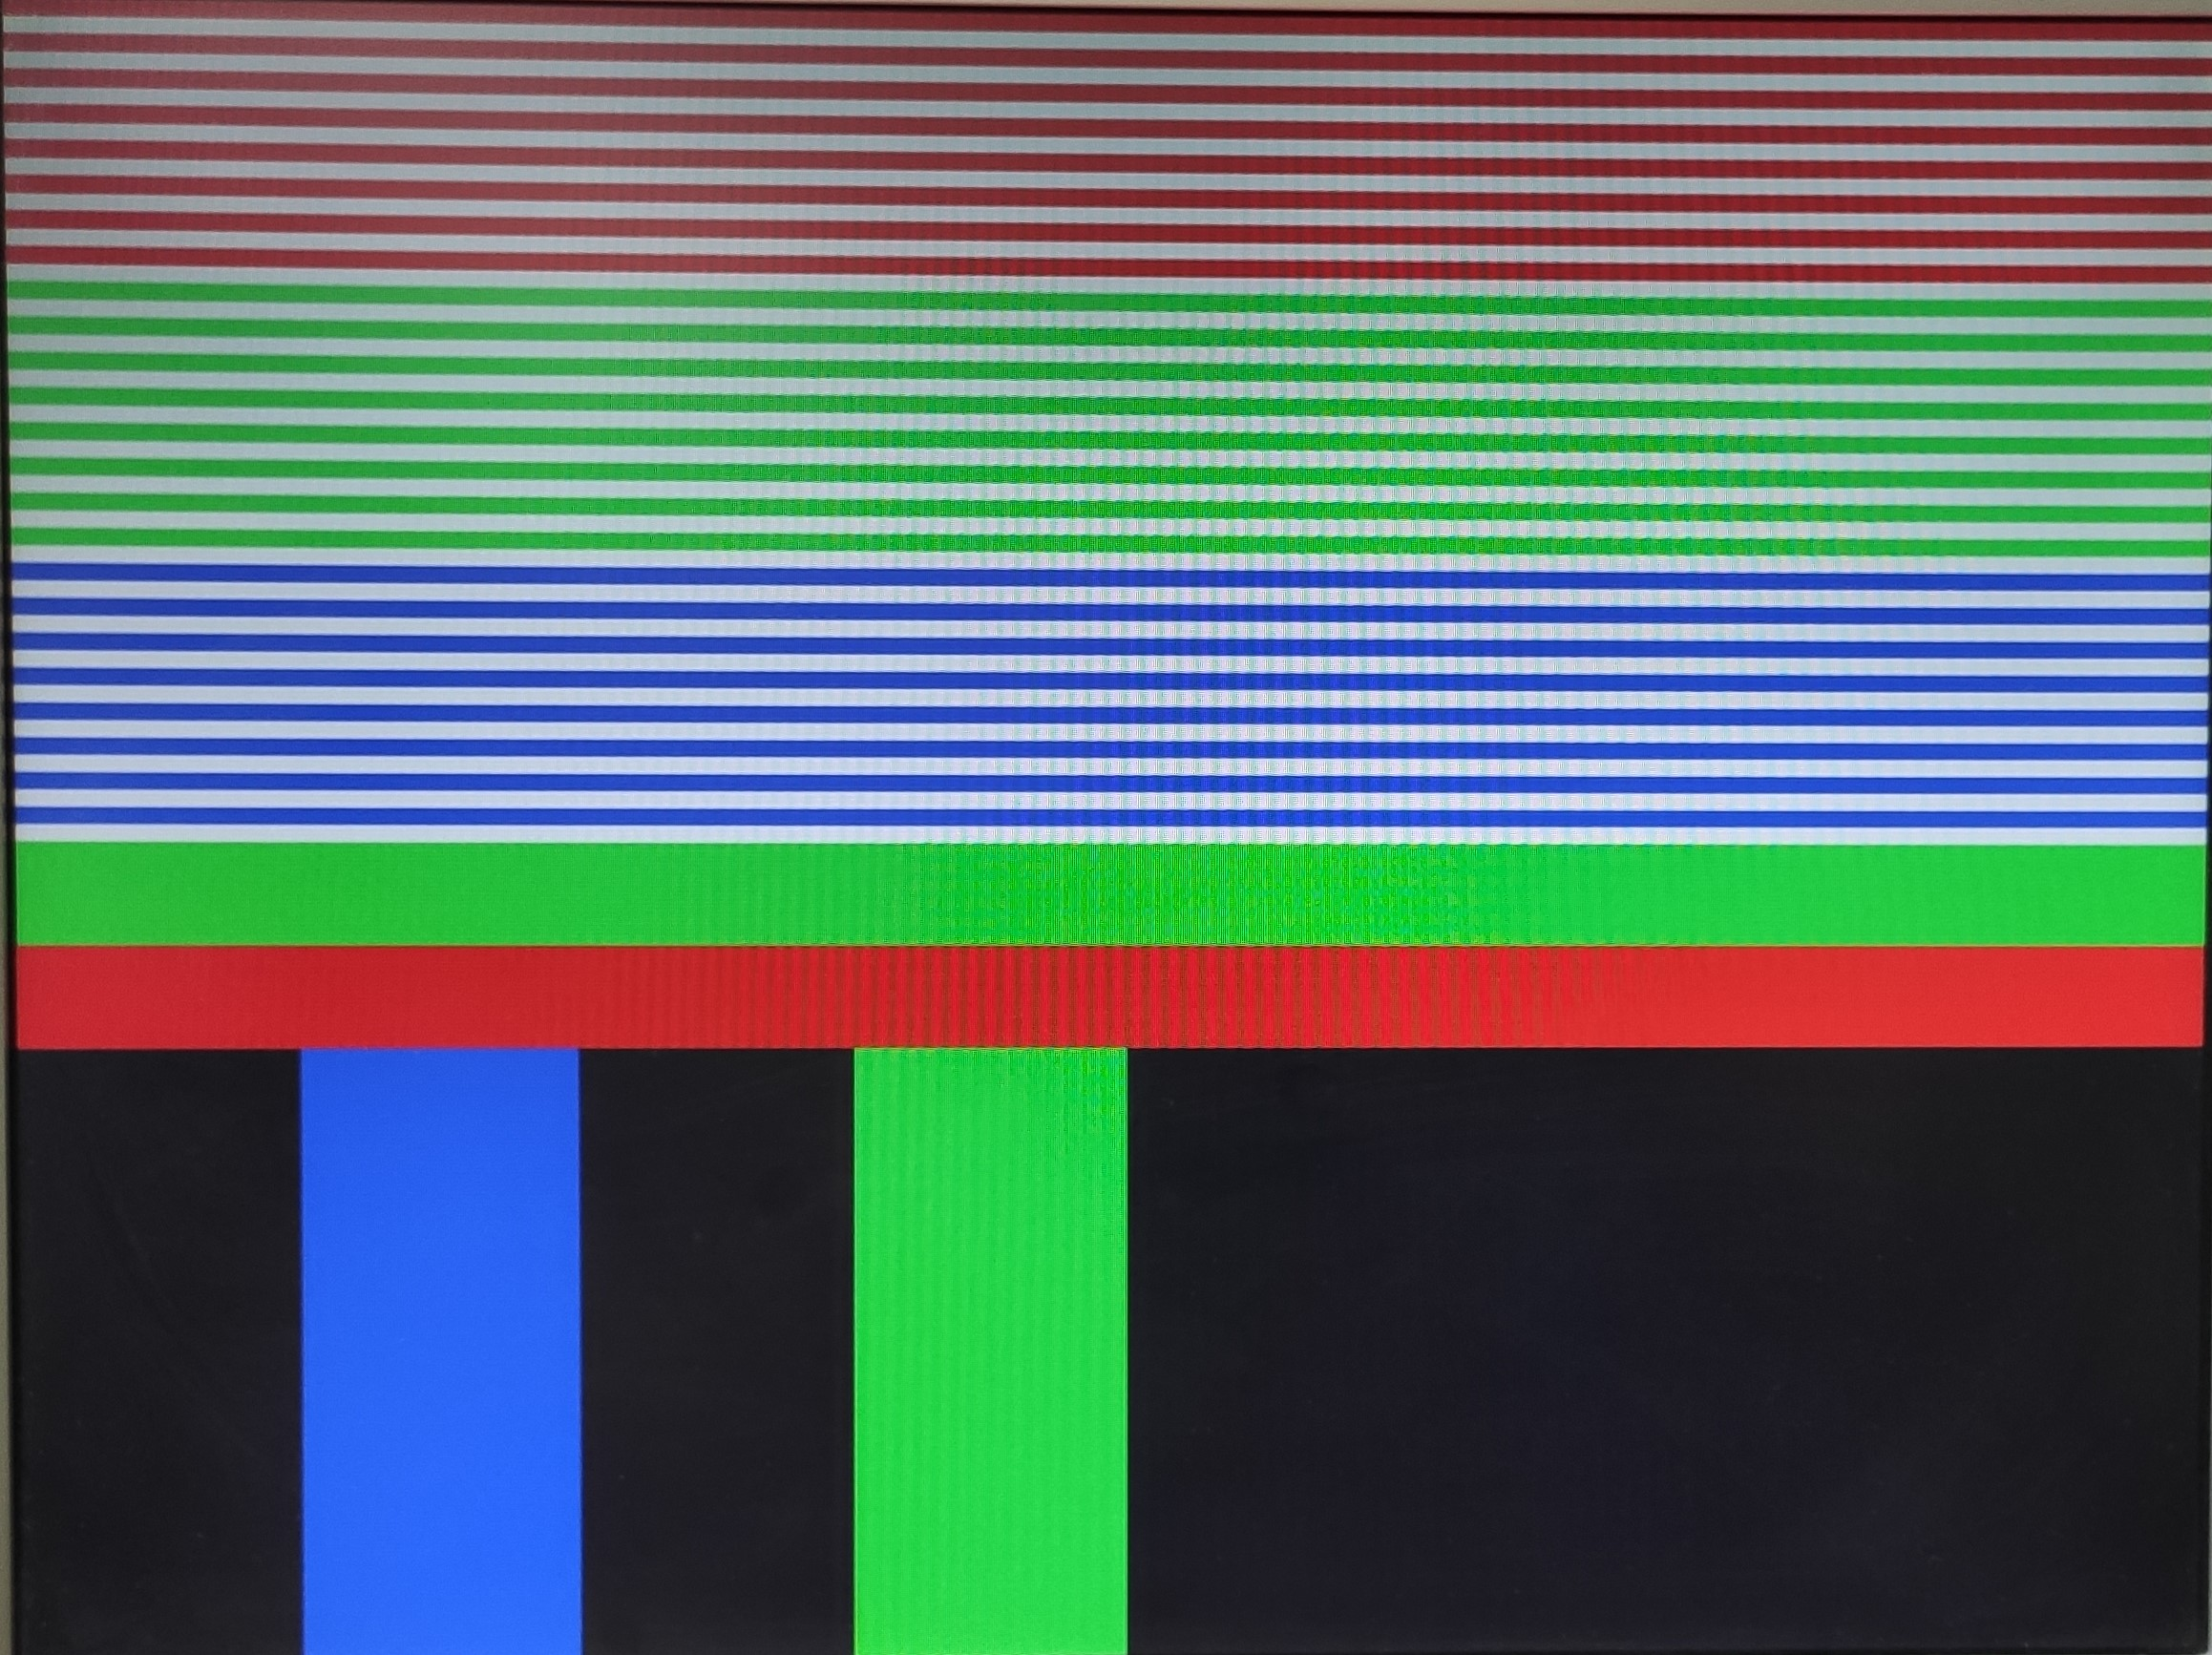
\includegraphics[width=0.5\textwidth]{pictures/picture cut} }
		\caption{picture example}
		\label{picture example}
	\end{figure}	
	
	Χρειάζεται να δημιουργήσουμε ένα module το οποίο ονομάζουμε VRAM στο οποίο τοποθετούμε τα instantiations για τις τρεις μνήμες (RGB) και δέχεται σαν input την διεύθυνση για να διαβάσει η μνήμη και σαν έξοδο τις τιμές των χρωμάτων. Από το manual για τις BRAM προκύπτει ότι για το συγκεκριμένο μέγεθος που επιλέξαμε χρειαζόμαστε διεύθυνση μεγέθους  14 bits. \\
	Παρακάτω παρατίθεται το Dataflow για το μέρος Α της εργασίας:
	\begin{figure} [H]
		\centering{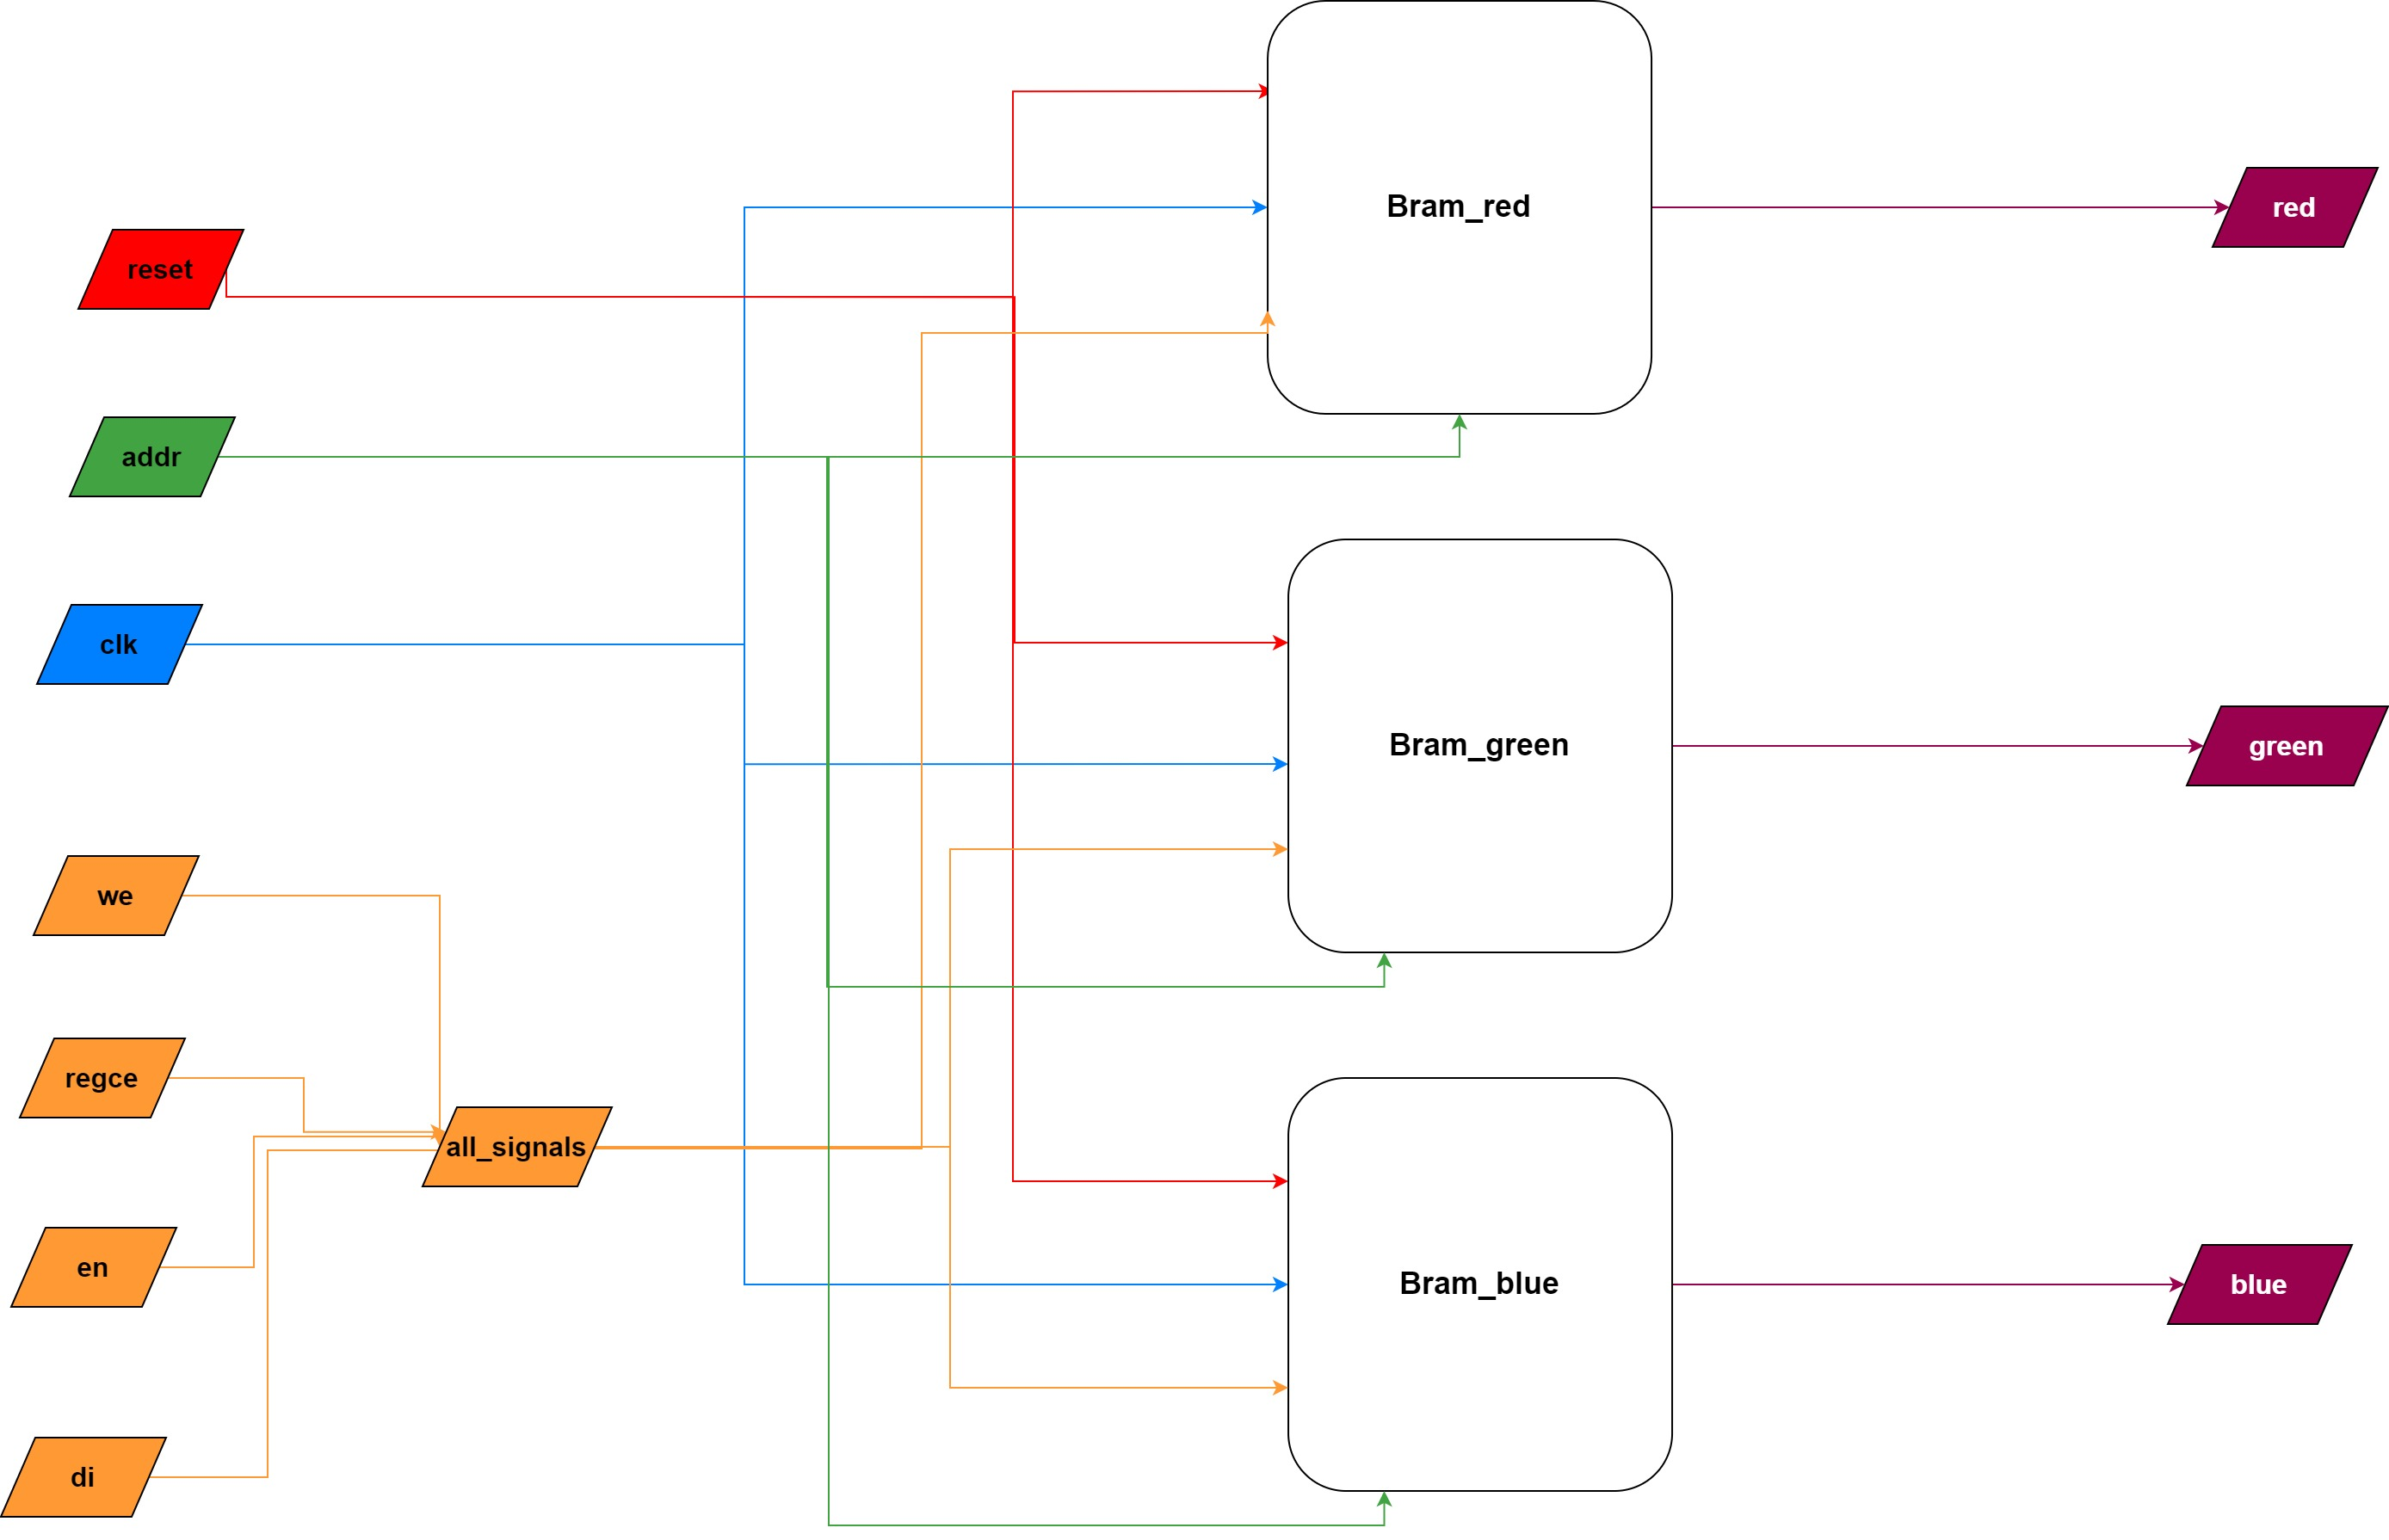
\includegraphics[width=0.8\textwidth]{../Lab3/partA/dataflow part A} }
		\caption{Dataflow VRAM}
		\label{Dataflow VRAM}
	\end{figure}
	
	
	
	
	
	\subsection{\textcolor{black}{Επαλήθευση VRAM} }
	Για την επαλήθευση του module της \verb*|VRAM| υλοποιούμε ένα πλαίσιο δοκιμής το οποίο ουσιαστικά, αλλάζει κάθε 100ns την τιμή της διεύθυνσης και με βάση το output που δέχεται εκτυπώνει το χρώμα που υπάρχει στην συγκεκριμένη διεύθυνση με βάση το σχήμα \ref{Colours combinations}. Οπότε, αρχικοποιώντας με συγκεκριμένες τιμές σε διάφορα σημεία την μνήμη, μπορούμε να ελέγξουμε εάν διαβάζει σωστές τιμές και στον σωστό χρόνο.\\ 
	Παρακάτω παρατίθεται ενδεικτικά ένα παράδειγμα του αποτελέσματος της προσομοίωσης για λίγες τιμές της μνήμης:
	
	\begin{figure} [htbp]
		\centering{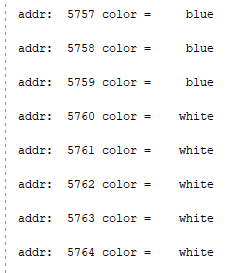
\includegraphics[width=0.4\textwidth]{pictures/simulation partA} }
		\caption{Simulation part A}
		\label{Simulation part A}
	\end{figure}

	\begin{figure} [htbp]
	\centering{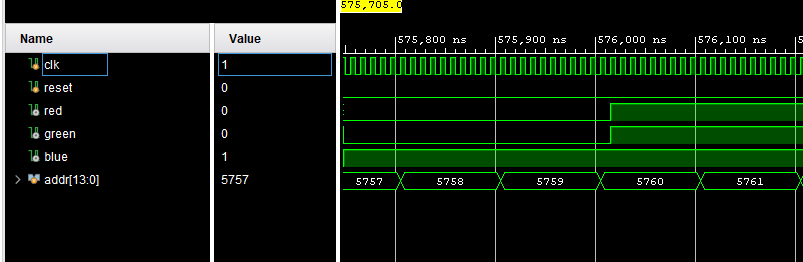
\includegraphics[width=0.5\textwidth]{pictures/kimatomorfes partA} }
	\caption{Kimatomorfes partA}
	\label{Kimatomorfes partA}
	\end{figure}
	Το συγκεκριμένο πλαίσιο δοκιμής θα μπορούσε να καλύπτει όλες τις περιπτώσεις και να αποφύγει κάθε είδους σφάλμα, εάν γινόταν έλεγχος για όλες τις τιμές, κάτι το οποίο είναι αδύνατο με το μάτι. Έγινε προσπάθεια για εξαγωγή των δεδομένων σε κάποιο αρχείο ώστε να γίνει πιο εύκολα έλεγχος, αλλά δεν επιτεύχθηκε. Τέλος, με στοχευμένες τιμές σε συγκεκριμένα σημεία της μνήμης καλύπτεται ένα αξιόλογο ποσοστό του testbench για την ορθότητα του \verb*|module_VRAM|.

	
	
	\section{\textcolor{cyan}{Μέρος Β - Υλοποίηση HSYNC και οριζόντιου μετρητή Pixel} }
	\subsection{\textcolor{black}{Περιγραφή υλοποίησης HSYNC}}
	Στο μέρος Β της εργασίας ζητείται η υλοποίηση του σήματος συγχρονισμού HSYNC το οποίο συγχρονίζει την οριζόντια διάσταση της οθόνης. Για τις οθόνες τύπου \verb|CRT| \verb*|(Cathode_Ray_Tube)| οι οποίες λειτουργούν με την χρήση ενός electron gun το οποίο εκτοξεύει ηλεκτρόνια σε κάθε pixel αναλόγως με το που βρίσκεται, είναι απαραίτητο να συγχρονίζεται ο οριζόντιος και ο κατακόρυφος άξονας και να ορίζονται οι χρόνοι που θα διανύει το electron gun την οθόνη.\\
	Ανάλογα με την ανάλυση και τον ρυθμό ανανέωσης που επιθυμούμε αλλάζουν οι χρόνοι του παλμού HSYNC καθώς και του οπτικού και μη διαστήματος. Για την ανάλυση των 640x480 pixels και 60Hz χρησιμοποιούμε τους χρόνους που δίνονται \href{http://tinyvga.com/vga-timing/640x480@60Hz}{\underline{εδώ}} με μία στρογγυλοποίηση για το ρολόι μας, οπότε προκύπτει ο παρακάτω πίνακας.
	
	\begin{figure} [htbp]
		\centering{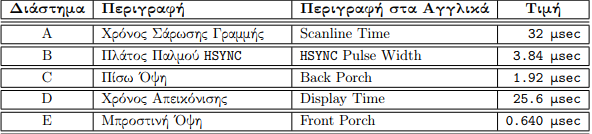
\includegraphics[width=0.6\textwidth]{pictures/horizontal timing} }
		\caption{Horizontal Timing}
		\label{Horizontal Timing}
	\end{figure}
	Οπότε χρειάζεται να υλοποιήσουμε ένα module το οποίο θα οδηγεί κατάλληλα το σήμα \verb*|HSYNC| και θα κρατάει σωστά τους χρόνους που χρειάζεται να εκτυπώνεται χρώμα στην οθόνη, καθώς επίσης και τις καθυστερήσεις για κάθε κατάσταση. Επιπλέον, κάθε στιγμή όταν βρισκόμαστε στο ενεργό σημείο της οθόνης θα πρέπει να γνωρίζουμε την ακριβή θέση, δηλαδή σε ποιο pixel της οθόνης, οπότε δημιουργούμε έναν μετρητή pixels \verb*|(hpixel)|.\\ Σημαντική σημείωση αποτελεί το γεγονός που αναφέραμε προηγουμένως, ότι δηλαδή θα πρέπει τα σήματα συγχρονισμού να κάνουν upscale την εικόνα καθώς από την ανάλυση των 128x96 που είναι αποθηκευμένα στην VRAM θα πρέπει να αποτυπώνεται 640x480. Οπότε χρησιμοποιώντας τον χρόνο \verb*|display_time| που δίνεται για την δεύτερη ανάλυση και διαιρώντας τα pixels του οριζόντιου άξονα που έχουμε στην διάθεση μας, επιτυγχάνουμε να εκτυπώνεται το ίδιο pixel σε 5 θέσεις στον ίδιο άξονα, προτού αλλάξει. Οπότε κάθε $25600/128 = 200 ns$ αλλάζει το ενεργό pixel, και εφόσον το διαθέσιμο ρολόι της FPGA είναι 10ns, ο μετρητής κάθε φορά που μετράει 19 (20 - 1 γιατί εφόσον είναι σε άλλο flip flop το hsync, η τιμή θα περάσει μετά από μία περίοδο) αυξάνει τον μετρητή \underline{hpixel}.
	Παρακάτω φαίνεται το Dataflow για το μέρους Β:
	\begin{figure} [H]
			\centering{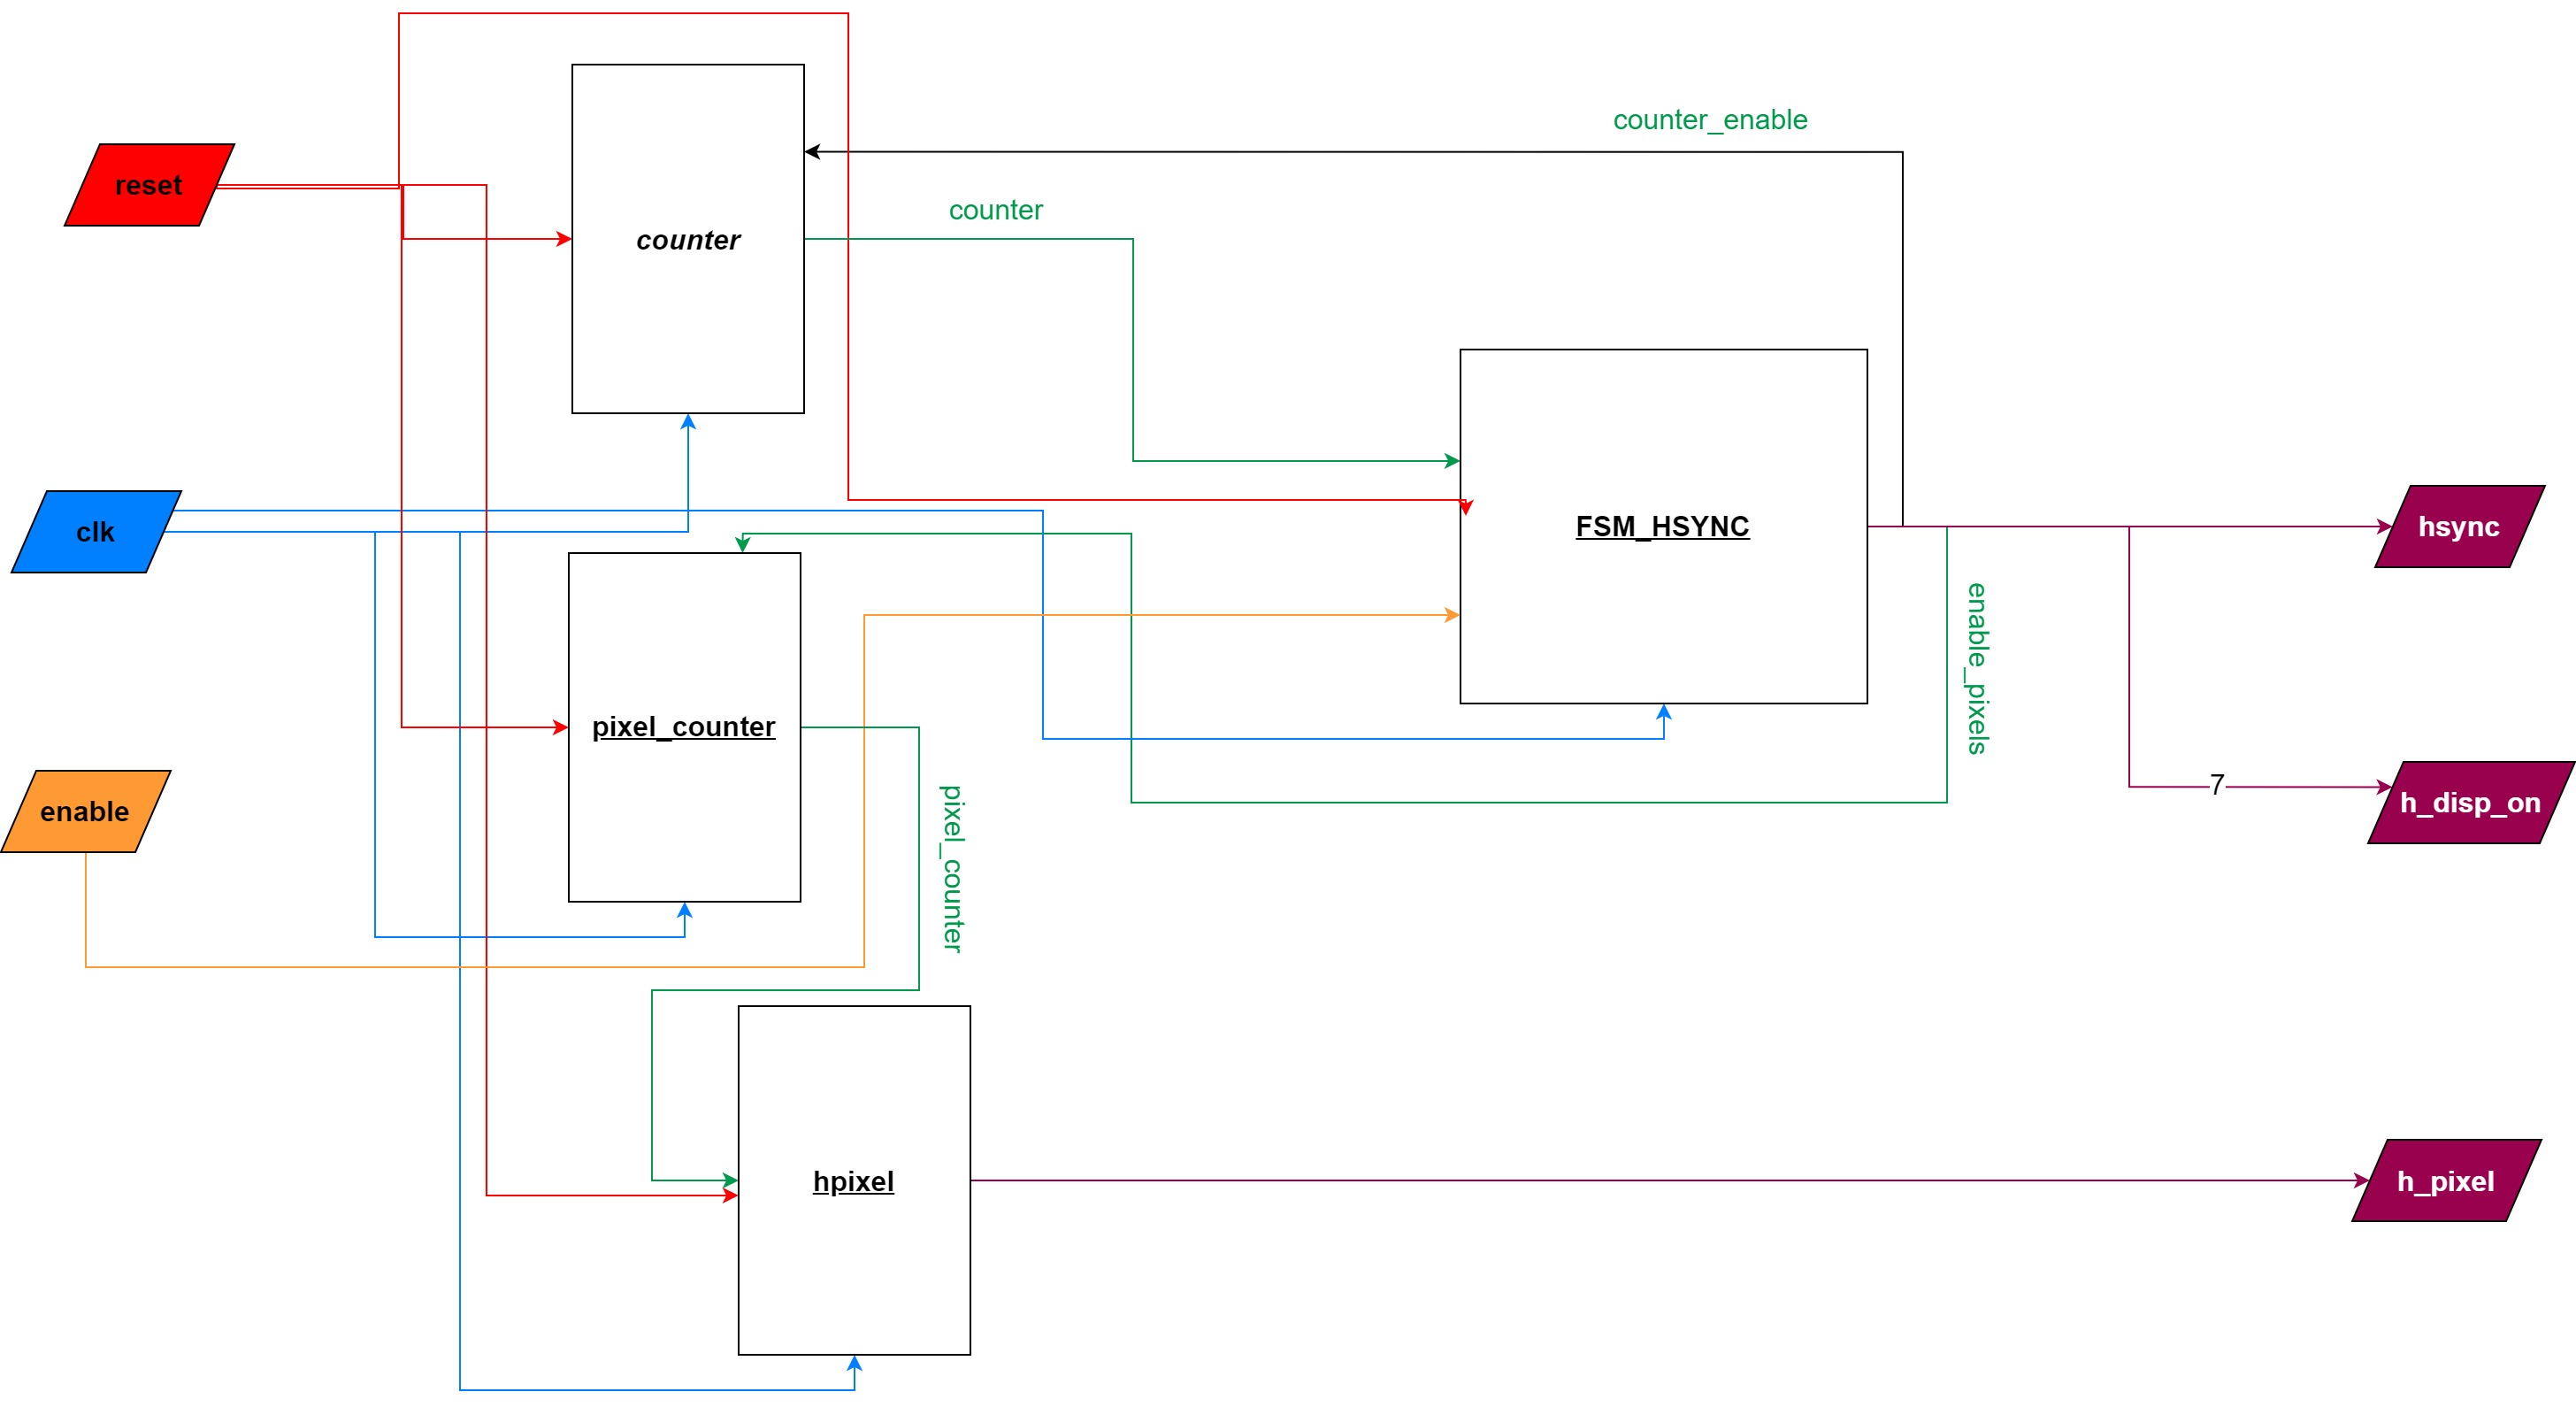
\includegraphics[width=0.8\textwidth]{../Lab3/partB/dataflow hsync} }
			\caption{Dataflow HSYNC}
			\label{Dataflow HSYNC}
	\end{figure}
	Τον έλεγχο των υπόλοιπων σημάτων και των καθυστερήσεων τον ελέγχουμε μέσω μίας FSM που αναλύεται παρακάτω.

	\subsubsection{\textcolor{black}{Υλοποίηση FSM HSYNC} }
	Η FSM που χρησιμοποιούμε είναι τύπου \verb*|Moore| και αποτελείται από 6 βασικές καταστάσεις. Οι 4 είναι εκείνες που δείχνουν πότε είναι σε ενεργό σημειό οθόνης και πότε όχι, ενώ μια αποτελεί την αρχική κατάσταση και μία άλλη την τελική όπου κάνει reset τον μετρητή.\\
	Αρχική κατάσταση αποτελεί η \verb*|off_state| όπου είναι κατάσταση αναμονής, περιμένει κάποιο σήμα enable ώστε να ξεκινήσει η λειτουργία και να περάσει στην επόμενη. Στην συνέχεια μεταβαίνουμε στην \verb*|width_pulse| όπου με το που ξεκινάει κατεβάζει το σήμα του HSYNC στο 0 και το κρατάει εκεί για όσο χρόνο αναφέρετε στο σχήμα \ref{Horizontal Timing}. Γενικότερα, η μετάβαση από την μία στην άλλη κατάσταση γίνεται μετρώντας τον χρόνο που χρειάζεται με έναν counter, έτσι επιτυγχάνεται κάθε κατάσταση να μπορεί να ελέγξει τα σήματα που χρειάζεται στον σωστό χρόνο. Στην συνέχεια έρχεται το \verb*|back_porch| όπου επαναφέρει το HSYNC στο 1 και μετά από 575 κύκλους ρολογιού προχωράει στο \verb*|display_time| όπου πλέον βρισκόμαστε στο ορατό κομμάτι της οθόνης οπότε πρέπει να ξεκινήσουμε να μετράμε pixels για να γνωρίζουμε την ακριβή μας θέση, για τον λόγο αυτό το συγκεκριμένο state στέλνει δύο σήματα ελέγχου που ενεργοποιεί τον counter για να ξεκινήσει την μέτρηση και για να ειδοποιήσει το controller ότι βρίσκεται σε ορατό κομμάτι. Στην συνέχεια μεταβαίνουμε στο \verb*|front_porch| όπου ξαναμηδενίζει τα δύο προηγούμενα σήματα και μετά από τον κατάλληλο χρόνο καταλήγει στο τελικό στάδιο \verb*|counter_reset| το οποίο απλά κάνει reset τον counter και επαναφέρει το σύστημα στο state \verb*|width_pulse|.\\
	\underline{Σημείωση} όλοι οι χρόνοι είναι -1 για να ληφθεί υπόψιν το γεγονός ότι καθυστερεί μία περίοδο μέχρι να μεταβεί στην επόμενη κατάσταση, και επιπλέον στο state \verb*|fornt_porch| είναι -2 διότι υπολογίζεται και ο χρόνος μετάβασης στο \verb*|counter_reset| και μετά στο \verb*|width_pulse|.
	Παρακάτω φαίνεται το διάγραμμα της FSM, όπου στην έξοδο φαίνονται μόνο τα μηνύματα όπου αλλάζουν σε κάθε κατάσταση και όχι όλα ώστε να είναι πιο ευανάγνωστο.
	\begin{figure} [htbp]
		\centering{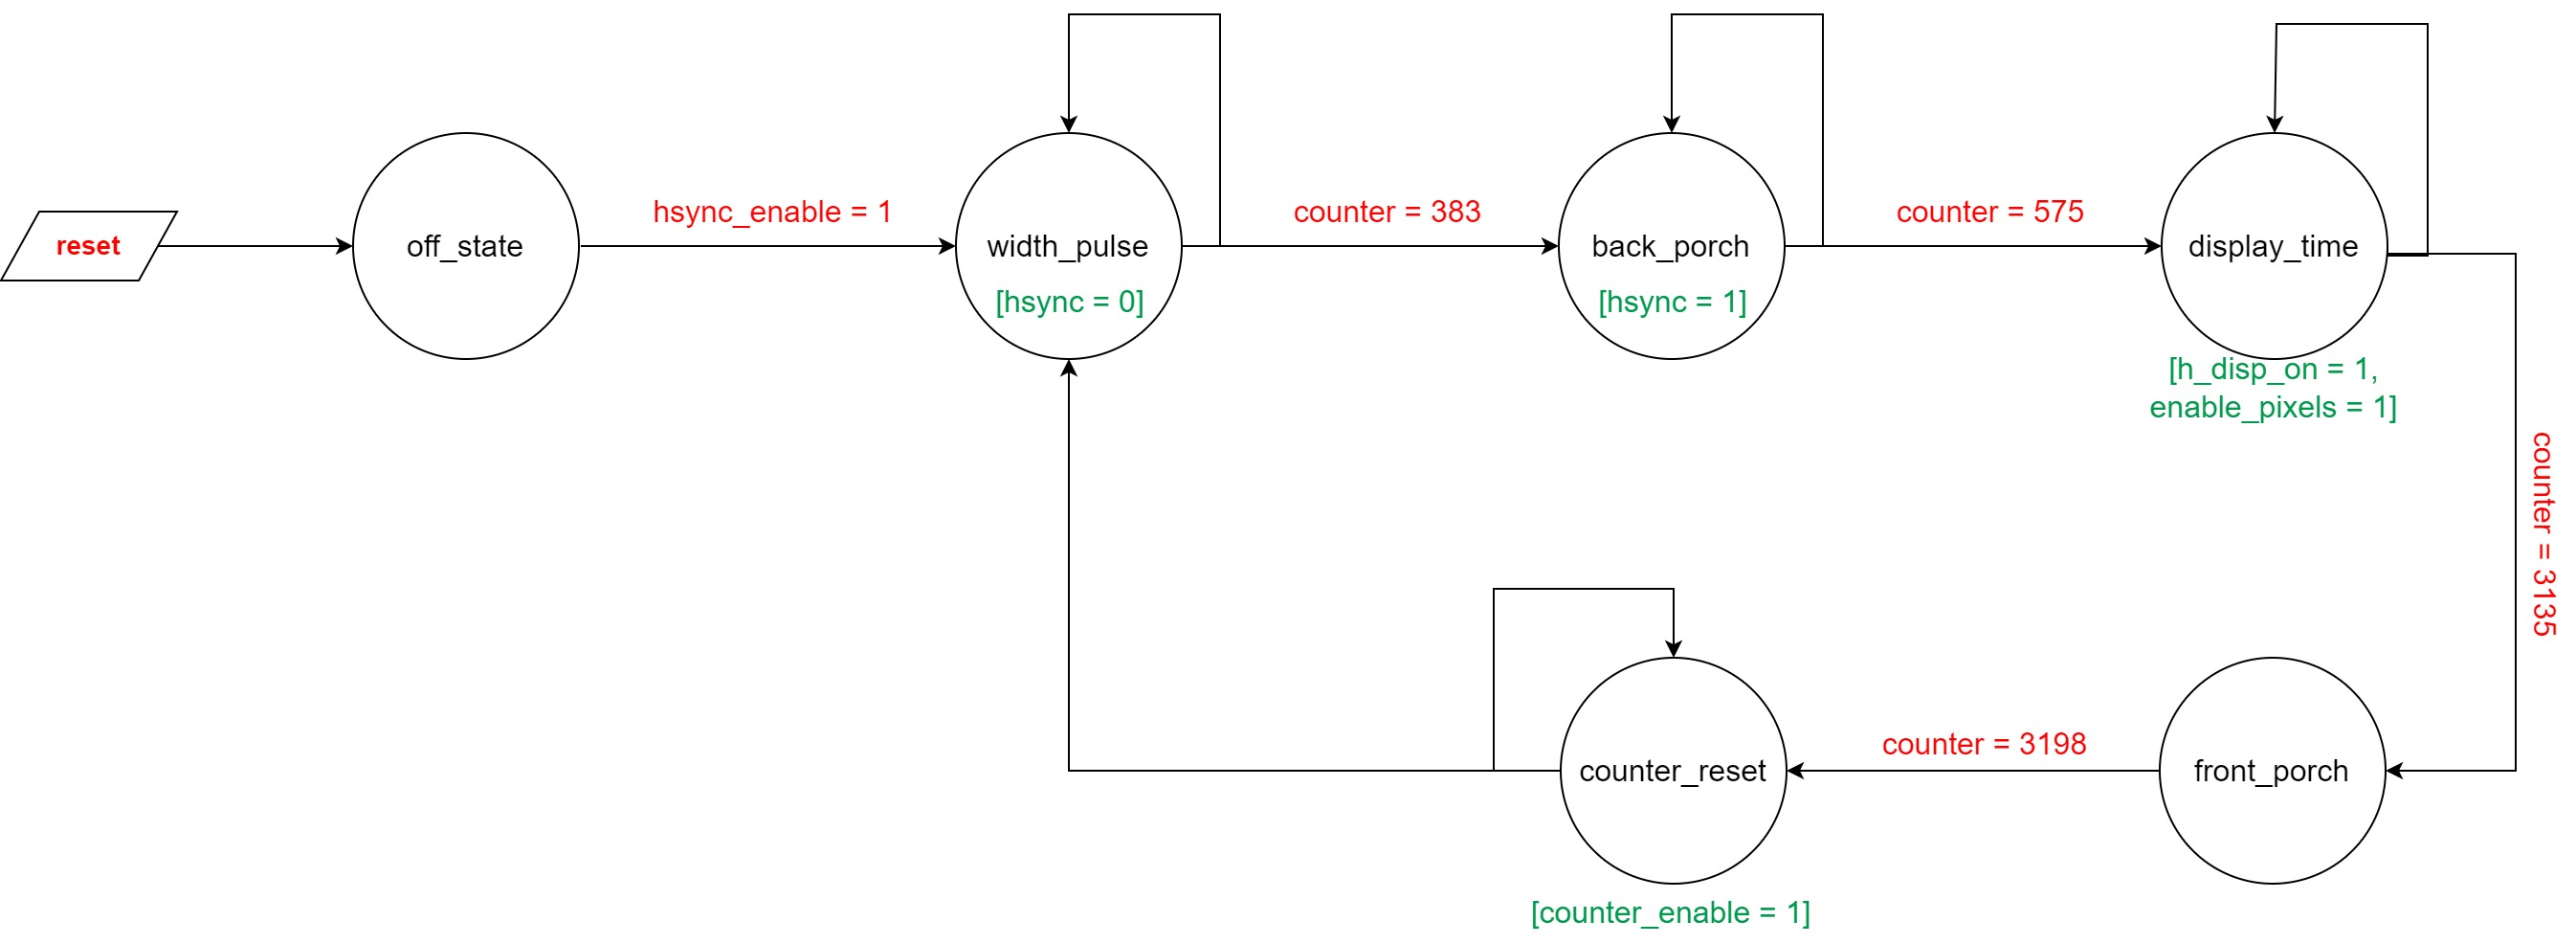
\includegraphics[width=\textwidth]{../Lab3/partB/FSM HSYNC} }
		\caption{FSM HSYNC}
		\label{FSM HSYNC}
	\end{figure}
	
	\subsubsection{\textcolor{black}{Always Blocks μέρος Β} }
	Στο module έχει υλοποιηθεί ένα always block ακολουθιακής λογικής και αποτελεί τον βασικό counter του συστήματος ο οποίος μετράει της περιόδους του ρολογιού και ορίζει στην FSM τον χρόνο για το πότε πρέπει να αλλάξει state. Επίσης ελέγχεται από την FSM για το πότε πρέπει να κάνει reset και να ξεκινήσει από την αρχή. Επιπλέον, υπάρχουν ακόμα δύο ακολουθιακά always blocks από τα οποία το πρώτο μετράει όπως αναφέρθηκε νωρίτερα, όταν βρισκόμαστε στο display time, 20 περιόδους και με βάση αυτό ο άλλος counter αυξάνεται κατά 1 και έτσι μπορούμε να μετράμε σε ποιο pixel βρισκόμαστε, δηλαδή το hpixel.
	
	\subsection{\textcolor{black}{Έλεγχος HSYNC} }
	Για να πετύχουμε έναν ικανοποιητικό έλεγχο για το μέρος Β, αρκεί να παρατηρήσουμε ότι οι χρόνοι για το κάθε state είναι σωστοί, ότι οι μεταβάσεις στις καταστάσεις γίνονται σωστά και τέλος ότι το hpixel μετράει σωστά τα pixels και φτάνει μέχρι το 127.\\
	Για να το πετύχουμε αυτό δημιουργούμε ένα πλαίσιο δοκιμής στο οποίο προσομοιώνουμε το ρολόι της FPGA αρχικοποιούμε τα κατάλληλα σήματα και τοποθετούμε το module HSYNC ώστε να προσομοιώσουμε την λειτουργία του.\\
	Στις παρακάτω κυματομορφές έχουν τοποθετηθεί marks στα αντίστοιχα σημεία αλλαγής κατάστασης ώστε να μπορεί να υπολογισθεί ο χρόνος εύκολα. Οι αλλαγές των καταστάσεων είναι εύκολα διακριτές από το σήμα \verb*|current_state| όπου μας δείχνει σε ποια κατάσταση βρισκόμαστε. Στην αριστερή εικόνα φαίνεται το μπροστινό κομμάτι της προσομοίωσης και υπολογίζοντας τους χρόνους αρχικά για τον παλμό HSYNC έχουμε $4.945 - 1105 = 3840ns$ που είναι όσο πρέπει, στην συνέχεια για το back porch έχουμε $6865 - 4945 = 1920 ns$ όπου επίσης είναι το επιθυμητό. Στην δεξιά εικόνα φαίνεται ένα μέρος από το πίσω κομμάτι της προσομοίωσης και σε συνδυασμό των δύο υπολογίζουμε τον χρόνο για το \verb*|display_time| όπου είναι $32465 - 6865 = 25600 ns$ το οποίο είναι σωστό. Τέλος υπολογίζουμε τον χρόνο για το \verb*|front_porch| όπου είναι $33105 - 32465 = 640 ns$ το οποίο είναι επίσης σωστό. Επίσης παρατηρούμε ότι αμέσως μετά ξεκινάει και πάλι ο παλμός για το HSYNC που σημαίνει ότι δεν έχουμε καθυστέρηση όταν ξεκινάει από την αρχή.


	%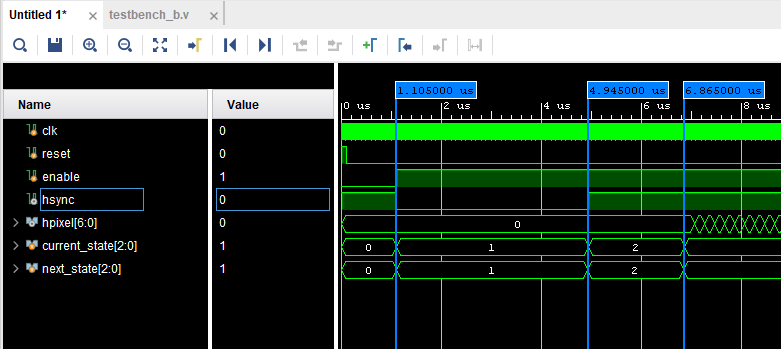
\includegraphics[width=0.5\textwidth]{pictures/mprosta kommati kimatomorfes}
	%	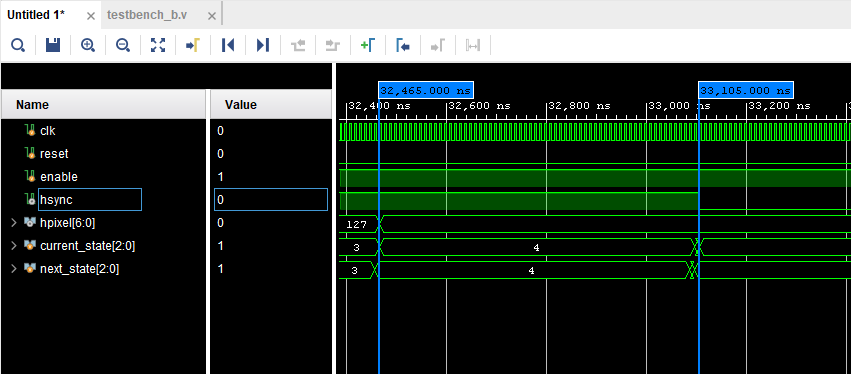
\includegraphics[width=0.5\textwidth]{pictures/piso kommati kimatomorfes}
		
		\begin{figure}[H]
			%\centering
			%\begin{minipage}{.5\textwidth}
				\centering
				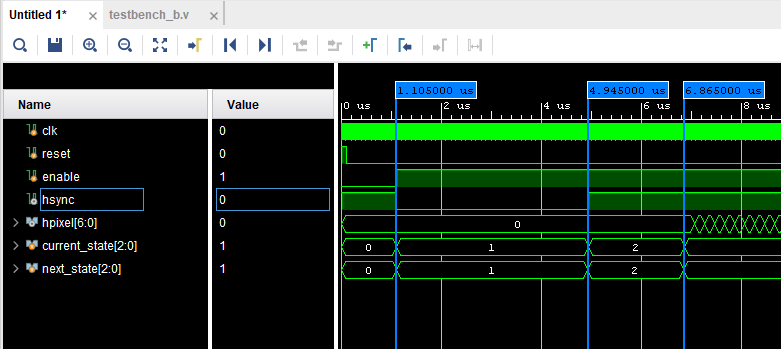
\includegraphics[width=.4\linewidth]{pictures/mprosta kommati kimatomorfes}
				\label{fig:test1}
			%\end{minipage}%
			%\begin{minipage}{.5\textwidth}
				\centering
				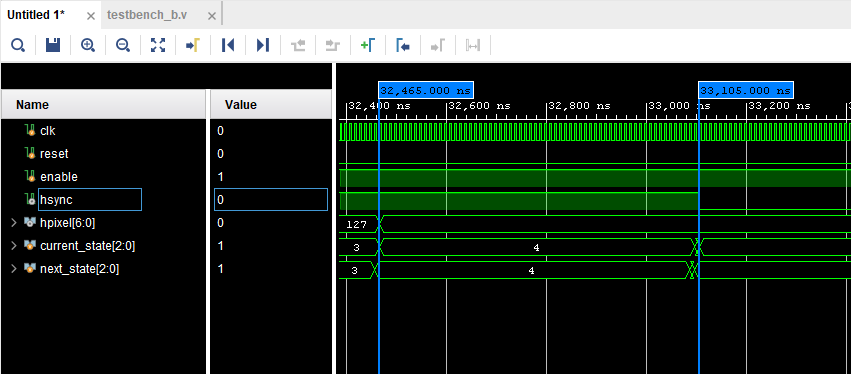
\includegraphics[width=.4\linewidth]{pictures/piso kommati kimatomorfes}
				\label{fig:test2}
			%\end{minipage}
		\end{figure}
	Ενώ παρακάτω φαίνεται η ολική προσομοίωση για το HSYNC:\\
	\begin{figure} [htbp]
		\centering{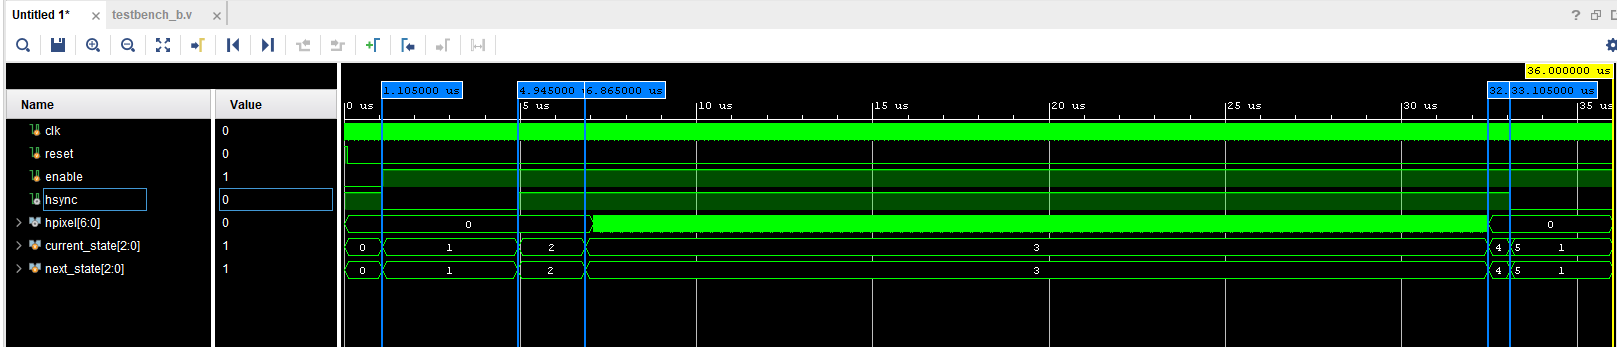
\includegraphics[width=\textwidth]{pictures/kimatomorfes part B} }
		\caption{Waveform HSYNC}
		\label{Waveform HSYNC}
	\end{figure}
	
	Στην συνέχεια θα πρέπει να επαναλάβουμε την διαδικασία για κάποιο χρονικό διάστημα μετά για να παρατηρήσουμε εάν ακόμα οι χρόνοι είναι σωστοί και ακολουθείται το ίδιο μοτίβο. Εφόσον κάνουμε αυτό μερικές φορές, τρέχουμε σύνθεση και implementation για το κύκλωμα μας και επιβεβαιώνουμε ότι δεν υπάρχουν latches και ότι οι αντίστοιχες προσομοιώσεις τρέχουν κανονικά. Πράγματι συμβαίνει αυτό με μοναδική εξαίρεση ότι στο timing simulation του implementation υπάρχουν μερικά spikes σε κάποια σήματα και κάποιες ελάχιστες καθυστερήσεις της τάξης των ps τα οποία είναι αμελητέα. Το testbench μας καλύπτει αρκετά για την λειτουργικότητα του κυκλώματος αλλά για να είμαστε πλήρως ασφαλείς θα έπρεπε να ελέγξουμε για μεγάλο χρονικό διάστημα κάθε επανάληψη του κυκλώματος και να επιβεβαιώσουμε την λειτουργία του, κάτι το οποίο είναι αδύνατο. Θα ήταν ιδανική η υλοποίηση ενός αυτόματου testbench αλλά ενώ έγινε προσπάθεια δεν επιτεύχθηκε να μετρηθούν σωστά οι χρόνοι χωρίς να βγαίνουν επιπλέον outputs από το module HSYNC.
	
	\section{\textcolor{cyan}{Μέρος Γ - Υλοποίηση VSYNC και Κατακόρυφου Μετρητή Pixel} }
	\subsection{Περιγραφή υλοποίησης VSYNC}
	Στο τρίτο μέρος της εργασίας ζητείται η υλοποίηση του σήματος συγχρονισμού VSYNC και η ολοκλήρωση της σύνδεσης του \verb*|VGA_controller|. Το σήμα VSYNC αποτελεί το σήμα για τον κατακόρυφο χρονισμό της οθόνης τύπου \verb*|CRT| και προσδίδει τους χρόνους που πρέπει να διασχισθεί ο κατακόρυφος άξονας καθώς και τα Hz στα οποία θα τρέξει. Όπως και προηγουμένως για τις συγκεκριμένες τιμές ανάλυσης και Hz προκύπτουν οι αντίστοιχοι χρόνοι που φαίνονται παρακάτω.
	\begin{figure} [htbp]
		\centering{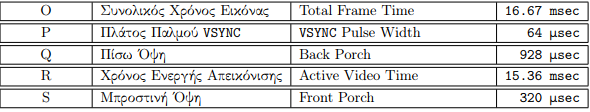
\includegraphics[width=0.7\textwidth]{pictures/Vertical timing} }
		\caption{Vertical Timing}
		\label{Vertical Timing}
	\end{figure}
	
	Ιδιαίτερη προσοχή χρειάζεται ώστε να μετρούνται ακριβώς οι χρόνοι και να συγχρονιστεί σωστά το display time του VSYNC με εκείνο του HSYNC. Για να το πετύχουμε αυτό στέλνουμε ένα σήμα enable από το VSYNC στο HSYNC σε κατάλληλο χρόνο ώστε να συμβαδίσουν οι ορατοί χρόνοι και των δύο. Για την υλοποίηση μας επίσης όπως και στο προηγούμενο μέρος χρησιμοποιούμε δύο counters για να μετράνε το \verb*|hpixel| και να γνωρίζουμε σε ποιο pixel του κατακόρυφου άξονα βρισκόμαστε. Με την ίδια διαδικασία για να πετύχουμε την επέκταση του κάθετου άξονα από 96 pixels της μνήμης σε 480, θα διαιρέσουμε το active video time με το 96, δηλαδή $15360000 / 96 = 160.000ns$ και το αποτέλεσμα είναι ο χρόνος που θα διαρκεί το κάθε κατακόρυφο pixel για να διαβάζουμε από την μνήμη την αντίστοιχη διεύθυνση. Παράλληλα το electron gun θα διανύει 480 pixels, οπότε θα παραμένει για πέντε σειρές στο ίδιο pixel στην μνήμη.\\
	Παρατίθεται το διάγραμμα ροής για το module \verb*|VSYNC_synchroniser|:
	\begin{figure} [H]
		\centering{\includegraphics[width=0.8\textwidth]{../Lab3/partC/dataflow Vsync} }
		\caption{Dataflow VSYNC}
		\label{Dataflow VSYNC}
	\end{figure}
	Για να υλοποιηθεί το VSYNC υλοποιούμε ένα module όπου περιέχει μία FSM που περιγράφει όλες τις καταστάσεις και ελέγχει τα σήματα, ενώ και τρεις counters όπου θα αναλυθούν παρακάτω. 
	\subsubsection{Υλοποίηση FSM VSYNC}
	Η FSM που χρησιμοποιήθηκε για το VSYNC είναι τύπου \verb*|Moore| και περιλαμβάνει 7 καταστάσεις, από τις οποίες οι 4 είναι για να πετύχουμε τους χρόνους που φαίνονται στον πίνακα \ref{Vertical Timing}. Η υλοποίηση της FSM γίνεται με δύο always blocks ένα ακολουθιακό για να αλλάζει τις καταστάσεις και ένα συνδυαστικό για να ελέγχει τα σήματα εξόδου.\\
	Πιο αναλυτικά για τις καταστάσεις, η αρχική κατάσταση είναι η \verb*|V_off| όπου είναι κλειστό το VSYNC και μόλις επανέλθει από το reset προχωράει στην επόμενη κατάσταση όπου είναι το \verb*|v_pulse_width| όπου το σήμα vsync γίνεται ίσο με 0 και η διάρκεια του συγκεκριμένου παλμού επιδεικνύει τα Hz που θα είναι η εικόνα. Στην συνέχεια προχωράμε στο state \verb*|v_back_porch| όπου επαναφέρει την τιμή του vsync στο 1, και ακολουθεί το \verb*|signal_for_hsync| όπου στέλνουμε ένα σήμα τύπου enable για να ξεκινήσει το hsync module και να συγχρονιστούν τα video time των δύο. Ο χρόνος μετάβασης στο \verb*|signal_for_hsync| προκύπτει από τον χρόνο για να μεταβούμε στο display time αφαιρόντας τα pulse-width, back-porch από το hsync, οπότε προκύπτει χρόνος ίσο με 986.240 ns. Στην συνέχεια μεταβαίνουμε στο \verb*|v_display_time| όπου στέλνει ένα σήμα enable για να ξεκινήσει να μετράει ο counter τα pixels και ένα ακόμα enable όπου επιδυκνύει στο controller ότι βρίσκεται στο video time. Ακολουθεί το state \verb*|v_front_porch| όπου επαναφέρει τα δύο αυτά σήματα στο 0 και τέλος το \verb*|v_reset_counter| όπου επαναφέρει τον counter στο 0 και επιστρέφει στο \verb*|v_width_pulse|.
	Αξίζει να σημειωθεί ότι όλοι οι χρόνοι για τις μεταβάσεις από το ένα state στο άλλο είναι οι χρόνοι που αναφέρονται παραπάνω διά 10 όπου είναι το ρολόι της FPGA για να συμβαδίζει με τον counter ο οποίος μετράει περιόδους. Επιπλέον, όλοι οι χρόνοι για τις μεταβάσεις είναι -1 περίοδο για να υπολογίζεται και ο χρόνος αλλαγής των registers. Εξαίρεση αποτελεί η μετάβαση στο \verb*|signal_for_hsync| καθώς είναι -2 περιόδους για να υπολογιστεί και ο χρόνος μετάβασης του hsync από το αρχικό του στάδιο στο \verb*|width_pulse|.\\
	Παρακάτω φαίνεται όλο το σχήμα για την FSM του VSYNC synchroniser:
	\begin{figure} [H]
		\centering{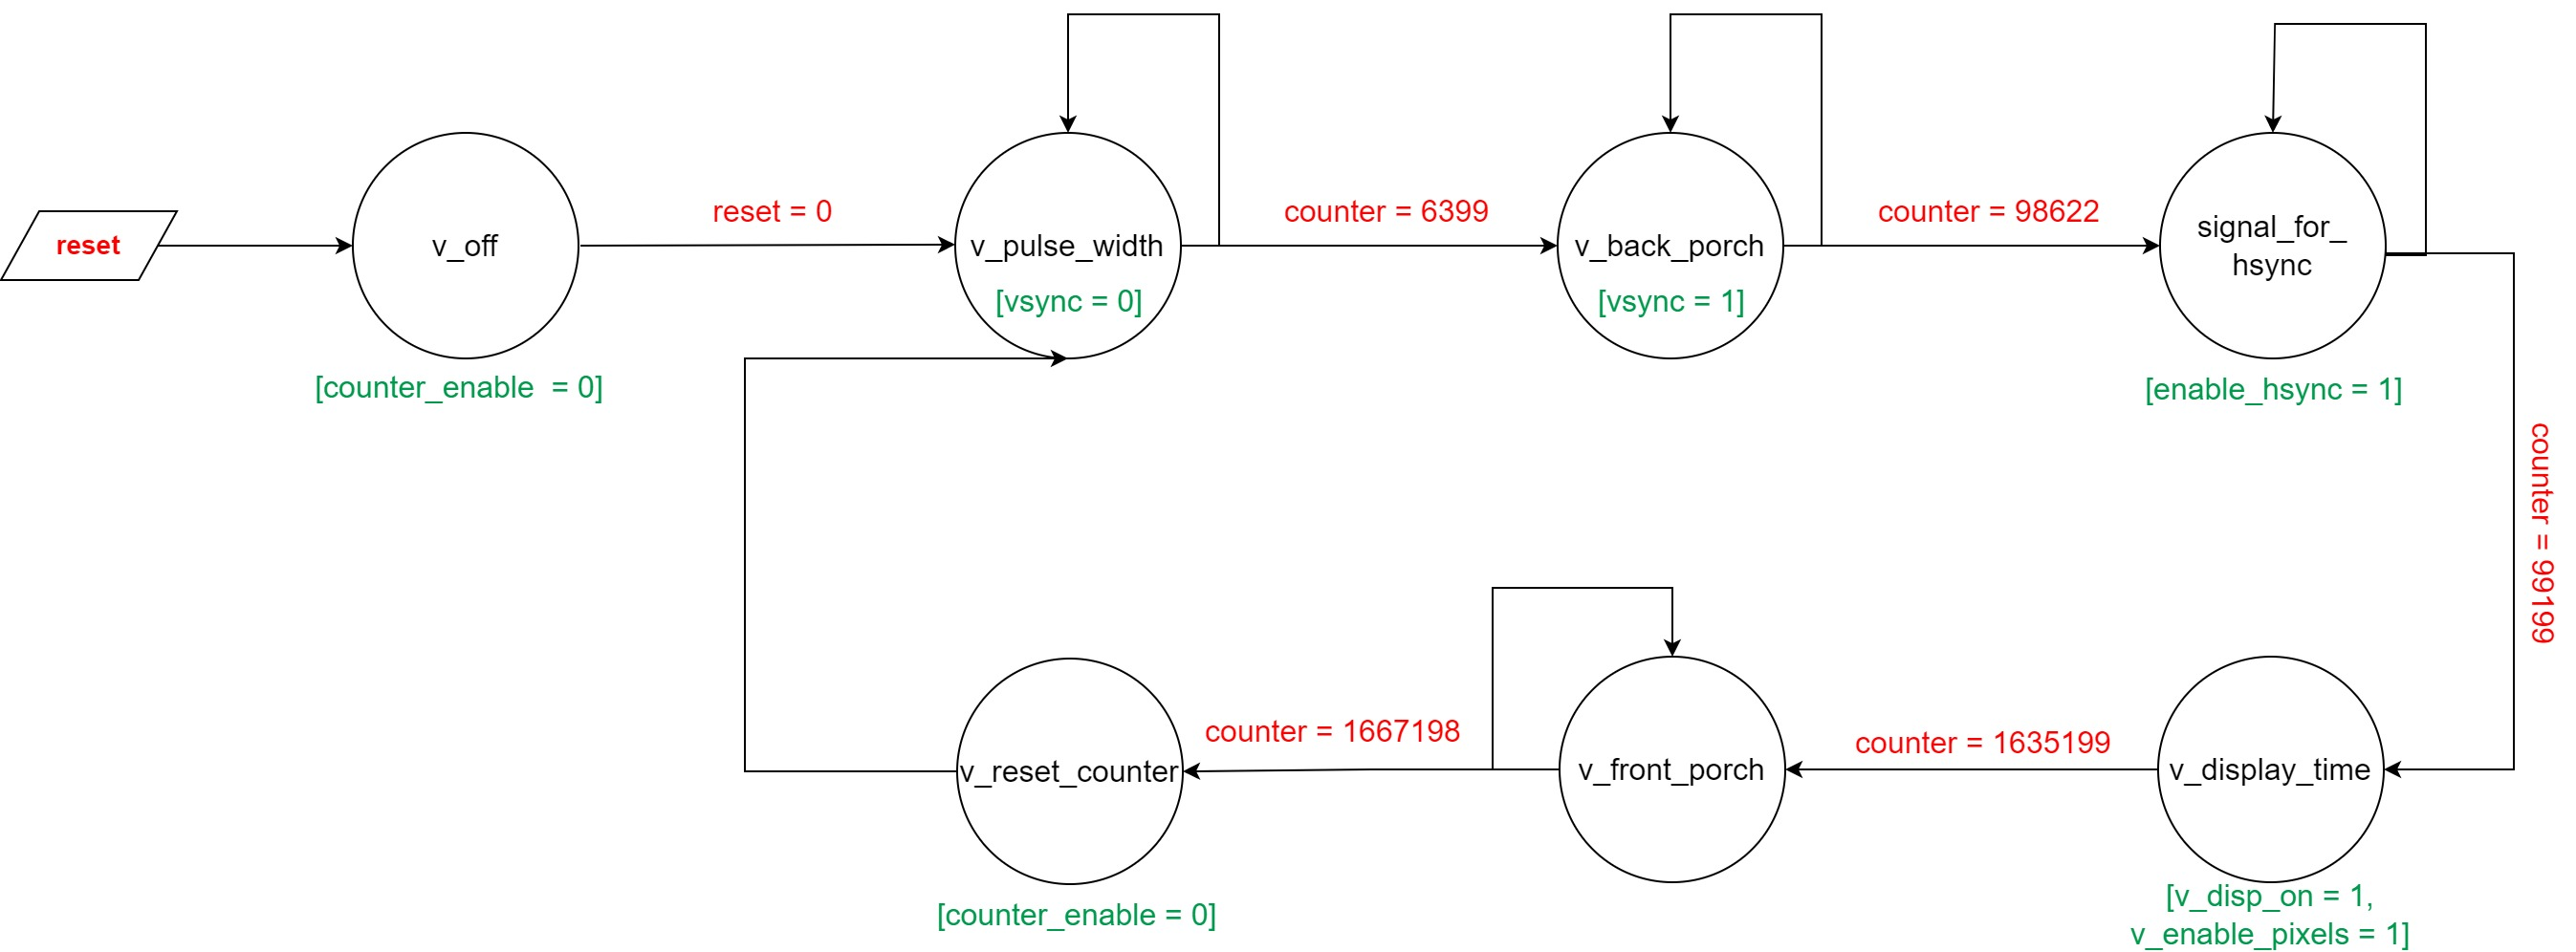
\includegraphics[width=\textwidth]{../Lab3/partC/FSM VSYNC} }
		\caption{FSM VSYNC}
		\label{FSM VSYNC}
	\end{figure}
	
	\subsubsection{Always blocks μέρος Γ}
	Για την υλοποίηση ολόκληρου του module χρησιμοποιήθηκαν τα αναγκαία always blocks για την FSM όπου αναφέρονται παραπάνω, ενώ επίσης και ένας counter όπου μετράει τις περιόδους του clock ώστε να μπορεί να μετρηθεί χρόνος για να γίνονται οι μεταβάσεις στην FSM. Επιπλέον υλοποιήθηκαν ακόμα δύο always blocks ακολουθιακής λογικής όπου το ένα μετράει 160.000ns και έχει και σήμα ελέγχου τύπου enable και το άλλο κάθε φορά που φτάνει σε αυτή την τιμή αυξάνεται κατά 1, ώστε να μετρούνται τα pixels του κάθετου άξονα της οθόνης. 
	
	\subsection{Έλεγχος VSYNC synchroniser}
	Για τον έλεγχο του VSYNC synchroniser ακολουθούμε την ίδια τακτική με το μέρος Β, οπότε δημιουργούμε ένα testbench με την ίδια λογική αλλά προσθέτουμε μέσα και το vsync και το hsync, για να ελέγξουμε και τον συγχρονισμό των δύο. Τρέχουμε την προσομοίωση για περίπου 16ms όσο η διάρκεια ενός frame και τα αποτελέσματα είναι τα εξής. Όπως φαίνεται και στις παρακάτω εικόνες για το vsync παλμό ισχύει ότι διαρκεί $64105 - 105 = 64000ns$, μέχρι το σημείο όπου στέλνετε το σήμα για ενεργοποίηση του HSYNC synchroniser  ισχύει $986335 - 64105 = 922230 ns$, ενώ για το back porch έχουμε $ 992105 - 64105 = 928.000 ns$. Στην συνέχεια υπολογίζουμε το v display time και προκύπτει ότι $ 16352105 - 986335 = 15365770 ns$ και τέλος ο χρόνος για το front porch είναι $16672105 - 16352105 = 320.000 ns$. Παρατηρούμε ότι όλοι οι χρόνοι είναι σωστοί και όπως θα έπρεπε.\\
	Παρακάτω φαίνονται όλες οι εικόνες για τους χρόνους:
	\begin{figure}[H]
		%\centering
		%\begin{minipage}{.5\textwidth}
		\centering
		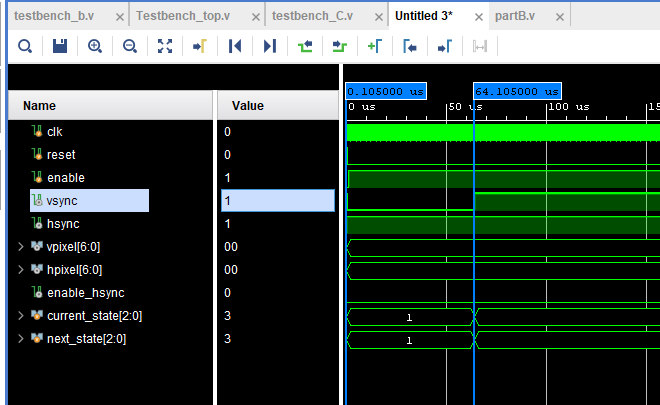
\includegraphics[width=.4\linewidth]{pictures/palmos vsync time}
		%\label{fig:test1}
		%\end{minipage}%
		%\begin{minipage}{.5\textwidth}
		\centering
		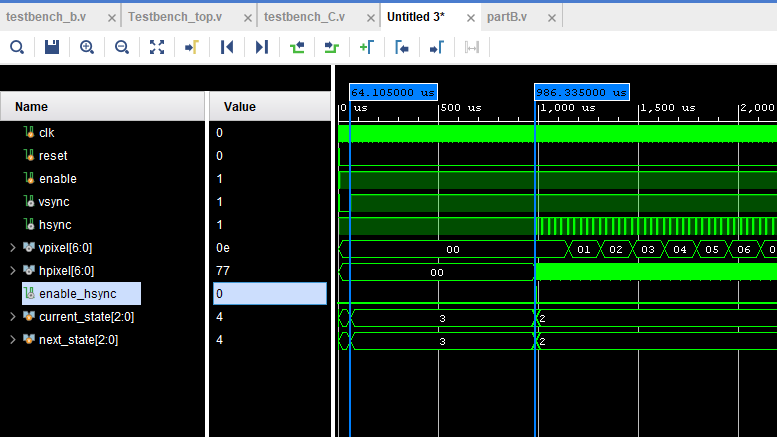
\includegraphics[width=.4\linewidth]{pictures/v back porch time}
	%	\label{fig:test2}
		%\end{minipage}
	\end{figure}

	\begin{figure}[H]
	%\centering
	%\begin{minipage}{.5\textwidth}
	\centering
	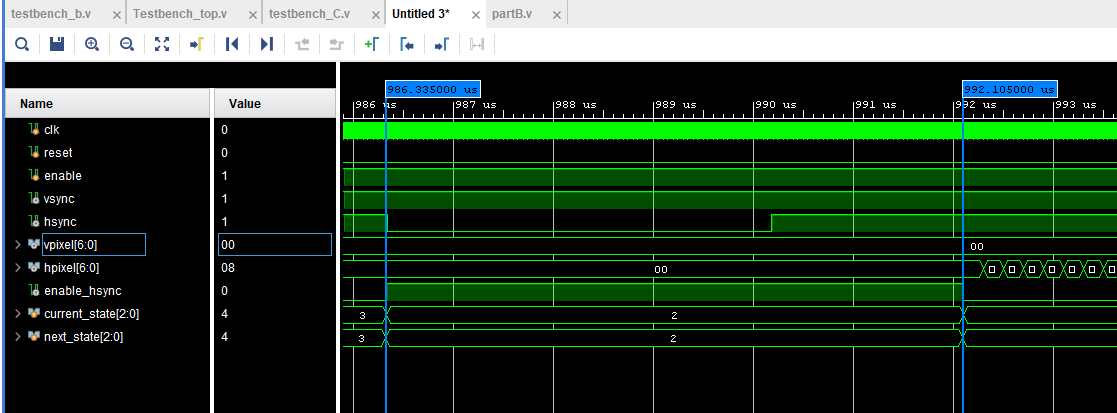
\includegraphics[width=.4\linewidth]{pictures/hsync enable time}
	%\label{fig:test1}
	%\end{minipage}%
	%\begin{minipage}{.5\textwidth}
	\centering
	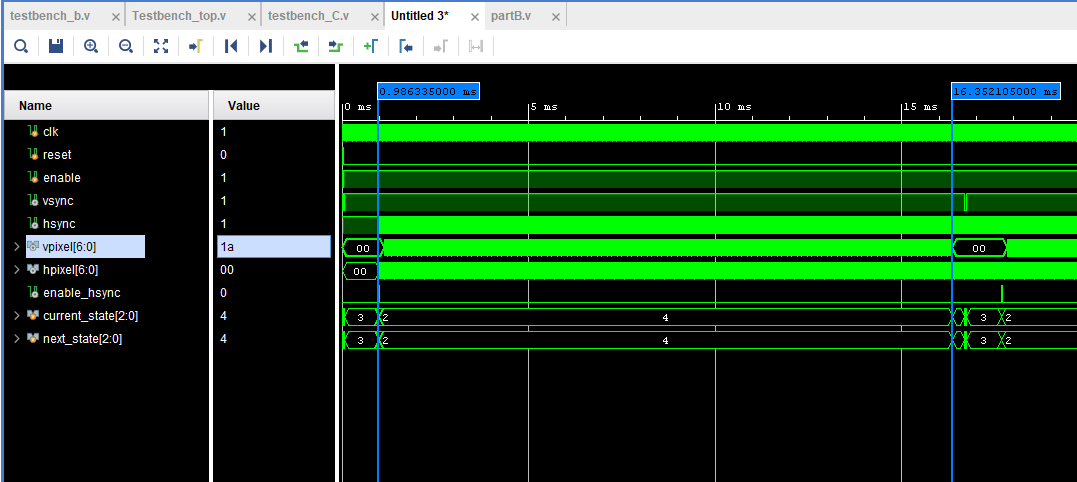
\includegraphics[width=.4\linewidth]{pictures/v display time}
	%	\label{fig:test2}
	%\end{minipage}
	\end{figure}

	\begin{figure}[H]
	\centering
	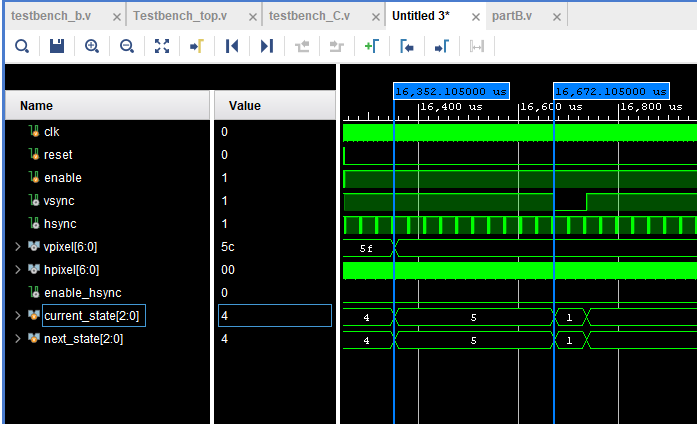
\includegraphics[width=.6\linewidth]{pictures/v front porch time}
	%	\label{fig:test2}
	%\end{minipage}
	\end{figure}

	Επιπλέον, παρατηρούμε από τις κυματομορφές και κοιτώντας τα current state των vsyn και hsync ότι είναι συγχρωνισμένα, δηλαδή ξεκινούν μαζί τα video time τους (state 4 για το vsync και 3 για το hsync), και θα συνεχίσουν να είναι έτσι συνεχώς. Αυτό φαίνεται και στην παρακάτω εικόνα:
	\begin{figure} [H]
		\centering{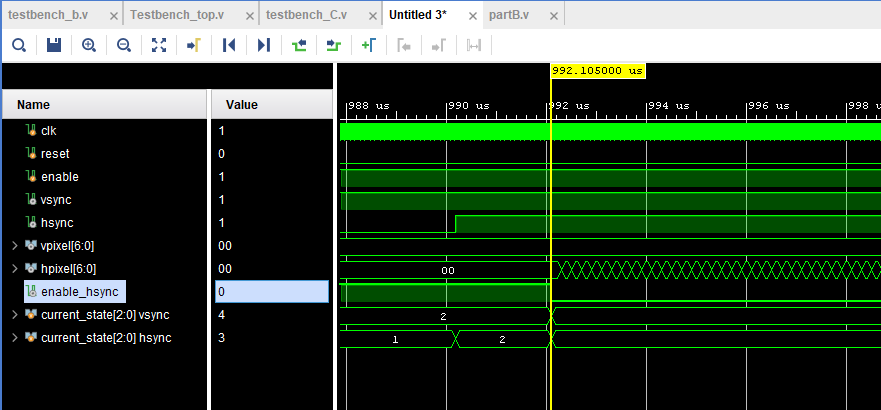
\includegraphics[width=0.7\textwidth]{pictures/vsync hsync synchronis} }
		\caption{VSYNC HSYNC synchronisation}
		\label{VSYNC HSYNC synchronisation}
	\end{figure}
	
	
	\subsection{Υλοποίηση VGA controller}
	Εφόσον ολοκληρωθεί το VSYNC synchroniser, μένει να συνδεθούν όλα μεταξύ τους και να γίνει έλεγχος. Οπότε δημιουργούμε το top module VGA controller και τοποθετούμε μέσα και τα τρία προηγούμενα modules: \verb*|VRAM|, \verb*|HSYNC_Synchroniser|, \verb*|VSYNC_Synchroniser|. Επίσης θέτουμε κάποια σήματα ελέγχου για την μνήμη στις τιμές που χρειάζεται με assign ώστε να λειτουργεί σωστά. Τα σήματα hpixel και vpixel γίνονται συνένωση σε ένα σήμα 14 bits το οποίο αποτελεί την ενεργή διεύθυνση της μνήμης όπου πρέπει να διαβάσουμε. Τέλος χρησιμοποιούμε ένα always block συνδιαστικής λογικής ώστε να ελέγχουμε πότε πρέπει να δείχνουμε σε ενεργή διεύθυνση στην μνήμη και πότε πρέπει να δείχνουμε σε σημείο της μνήμης (14'd16128) όπου είναι R=G=B=0, με βάση τα σήματα που μας λένε ότι βρίσκεται και το vsync και το hsync σε video time.\\
	Πααρακάτω φαίνεται το Dataflow για όλο το \verb*|VGA_Controller|:
	\begin{figure} [H]
		\centering{\includegraphics[width=0.8\textwidth]{../Lab3/top/dataflow top module} }
		\caption{Dataflow VGA Controller}
		\label{Dataflow VGA Controller}
	\end{figure}
	
	\subsection{Έλεγχος VGA Controller}
	Για τον έλεγχο του VGA controller χρησιμοποιούμε ένα πλαίσιο δοκιμής με παρόμοια λογική με τα προηγούμενα, αλλά αυτή την φορά προσθέτουμε μέσα το top module ώστε να παρατηρήσουμε ότι όλο το κύκλωμα μαζί λειτουργεί σωστά. Εφόσον έχει ελεγχθεί ότι οι χρόνοι των σημάτων είναι σωστοί και ο συγχρονισμός των VSYNC και HSYNC επίσης, το μόνο που μένει να παρατηρήσουμε είναι εάν αλλάζει σωστά η διεύθυνση όταν πρέπει και βγάζει και την σωστή τιμή και εάν στον κενό χρόνο αποτυπώνεται μαύρο χρώμα.\\
	Οπότε αρκεί να παρατηρήσουμε ότι όταν βρίσκεται στο video time και τα δύο σήματα, μόνο τότε το addr παίρνει τιμή και αυξάνεται κανονικά, ενώ όταν δεν είναι ενεργό δείχνει στην διεύθυνση 16128 όπου το χρώμα είναι μαύρο. Επίσης παρατηρούμε ότι το addr φτάνει μέχρι την σωστή τιμή των 12.287 pixels και μετά κάνει reset.
	\begin{figure}[H]
		%\centering
		%\begin{minipage}{.5\textwidth}
		\centering
		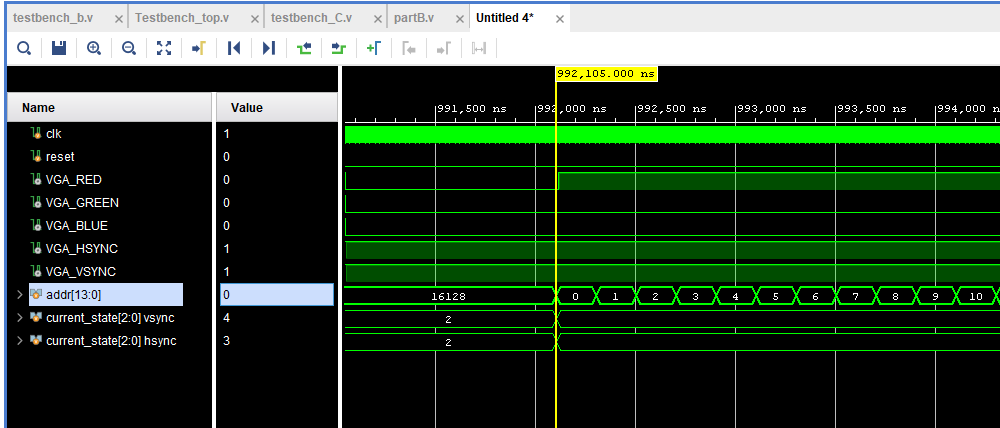
\includegraphics[width=.4\linewidth]{pictures/addr test}
		%\label{fig:test1}
		%\end{minipage}%
		%\begin{minipage}{.5\textwidth}
		\centering
		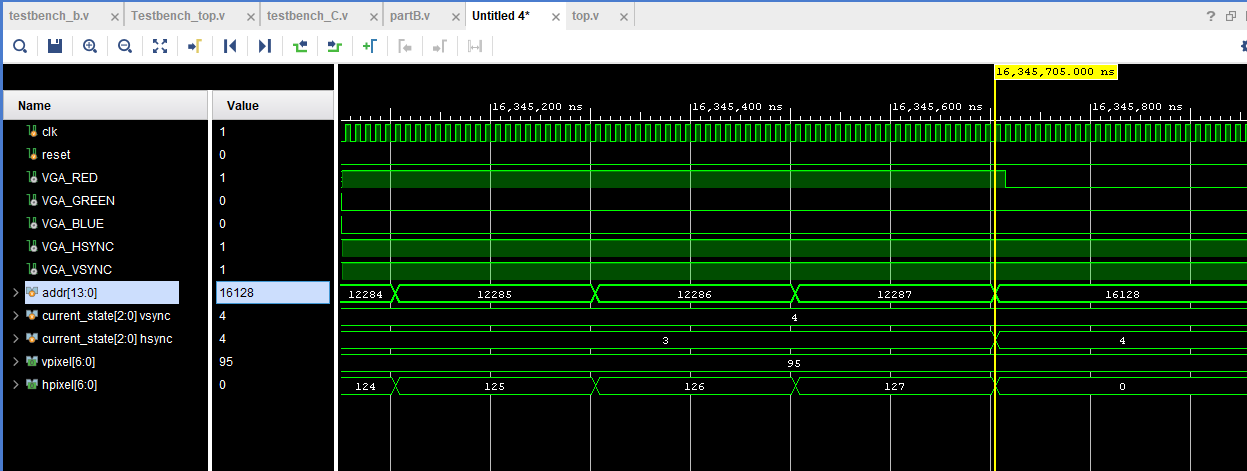
\includegraphics[width=.4\linewidth]{pictures/final addr value}
		%	\label{fig:test2}
		%\end{minipage}
	\end{figure}
	
	\begin{figure}[H]
		\centering
		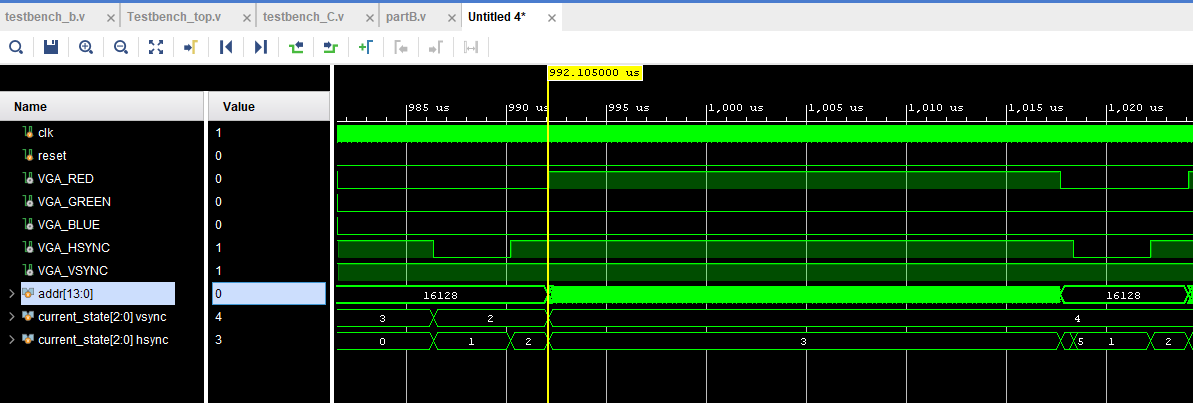
\includegraphics[width=.6\linewidth]{pictures/addr full}
		%	\label{fig:test2}
		%\end{minipage}
	\end{figure}
	Εφόσον ελεγχθεί σωστά και το ολικό κύκλωμα, το περνάμε από σύνθεση και implementation όπου τρέχουμε και πάλι προσομοιώσεις και εφόσον είναι σωστές προχωράμε στα παρακάτω βήματα.\\
	Τα μόνα warnings που παρουσιάζονται μετά την σύνθεση και το implemntation είναι για την μνήμη, όπου δεν χρησιμοποιούμε όλες τις τιμές που πρέπει καθώς εμείς μόνο διαβάζουμε και δεν γράφουμε από την μνήμη. Μετά από έλεγχο στο internet διαπιστώθηκε ότι δεν μας επηρεάζει κάπως στο κύκλωμά μας.
	
	\section{\textcolor{cyan}{Πείραμα στην πλακέτα FPGA}}
	
	Εφόσον είχε υλοποιηθεί όλο το κύκλωμα και σε επίπεδο προσομοίωσης λειτουργούσε, έμενα να γίνει έλεγχος και στην πλακέτα. Αρχικά, δημιουργήσαμε το αρχείο XDC με τους περιορισμούς για την πλακέτα και για να ορίσουμε τα pins για τα inputs και outputs της πλακέτας. Η διαδικασία ήταν απλή καθώς απλά διαβάζοντας το manual για την πλακέτα υπάρχει μία εικόνα που δείχνει ακριβώς ποια pins πρέπει να συνδεθούν.
	\begin{figure} [H]
		\centering{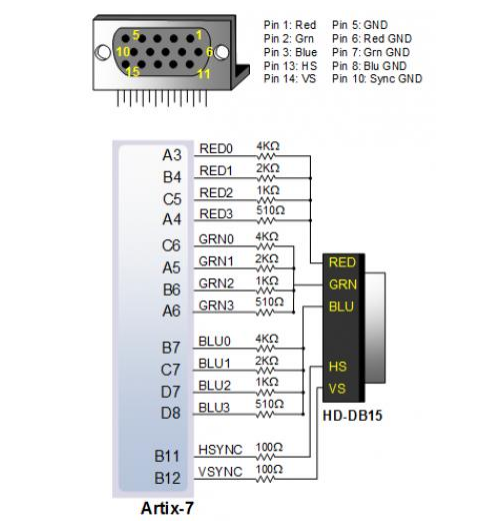
\includegraphics[width=0.6\textwidth]{pictures/vga manual} }
		\caption{VGA manual}
		\label{VGA manual}
	\end{figure}
	Σημαντικό είναι να συνδεθούν σε όλα τα inputs της πλακέτας για κάθε χρώμα η έξοδος από το κύκλωμα μας για το αντίστοιχο χρώμα. Δηλαδή και στα 4 πινάκια για κάθε χρώμα βάζουμε την ίδια έξοδο π.χ \verb*|VGA_RED|.\\
	Όταν έγινε ο έλεγχος στην πλακέτα στην αρχή ενώ είχα σταθερή εικόνα και όχι βίντεο και ζωγραφιζόταν το σχέδιο που ήθελα στην οθόνη, κάθε φορά δεν εμφανιζόταν ένα χρώμα και αρχικά ήταν το κόκκινο. Μετά από κάποιες αλλαγές στην VRAM δεν εμφανιζόταν το πράσινο. Οπότε κατάλαβα ότι μάλλον κάτι είναι λάθος με την vram. Έτσι ξανά έκανα το σχέδιο από την αρχή για τις αρχικοποιήσεις της VRAM, ενώ πρόσθεσα και στήλες για να είμαι σίγουρος ότι δεν ήταν βίντεο. Επίσης παρατήρησα στην προσομοίωση ότι αντί να δείχνει στον νεκρό χρόνο σε χρώμα μάυρο έδειχνε σε κόκκινο, και το άλλαξα αλλάζοντας απλά την διεύθυνση της μνήμης. Μετά από αυτές τις αλλαγές στην επόμενη προσπάθεια έπαιξε κανονικά και φαινόταν ακριβώς η εικόνα που ήθελα. Οπότε είτε έφταιγε το ότι έδειχνε κόκκινο σε νεκρό χρόνο και κάπως το επηρέαζε, είτε είχε γίνει κάποιο λάθος στην αρχικοποίηση της vram (ίσως παραπάνω θέσεις από λάθος).\\
	\textbf{Παρατίθεται φωτογραφεία από την στιγμή που δούλεψε στην πλακέτα!}
	\begin{figure} [H]
		\centering{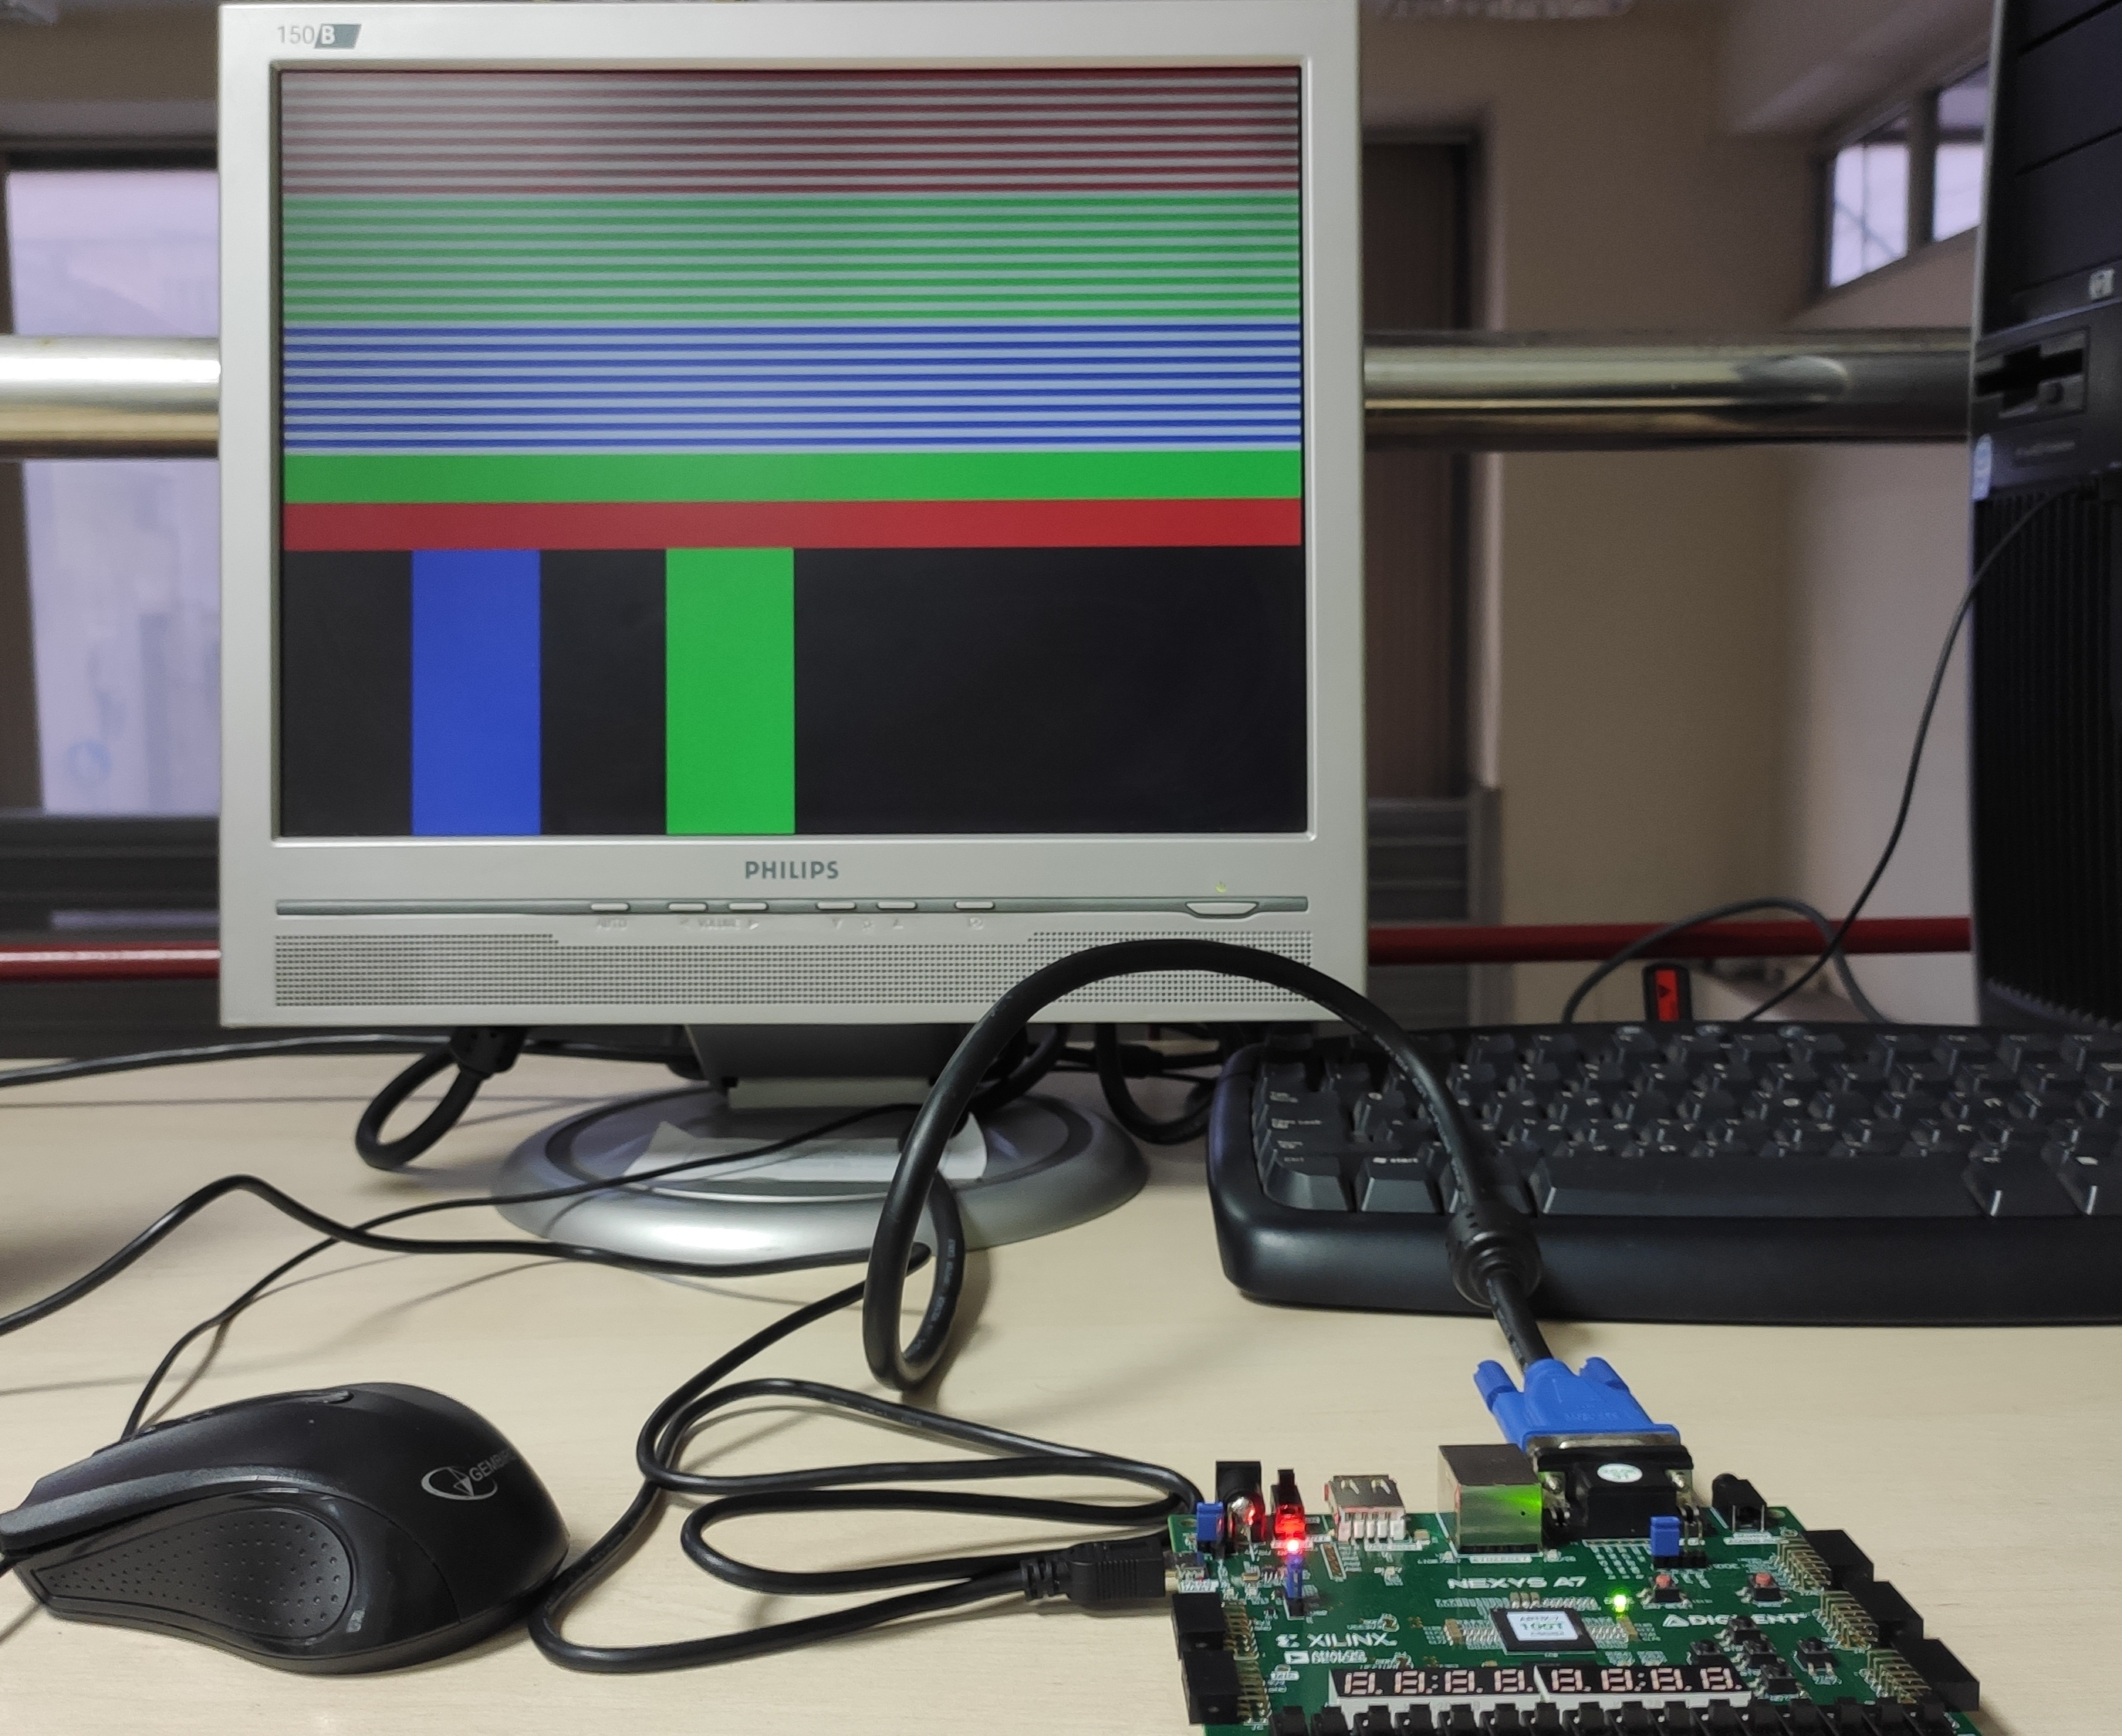
\includegraphics[width=0.7\textwidth]{pictures/test on fpga} }
		\caption{Test on FPGA}
		\label{Test on FPGA}
	\end{figure}
	
	
	\section{\textcolor{cyan}{Συμπεράσματα}}
	Γενικά το VGA Controller αποτελούσε μία αρκετά απαιτητική εργασία, όπου χρειαζόταν ιδιαίτερη προσοχή διότι ακόμα και ns να έχανες σε χρόνο ήταν πολύ πιθανό είτε να μην έχεις σταθερή εικόνα, είτε να μην ανάβει καθόλου η οθόνη. Θεωρώ ότι έγινε μία αρκετά ικανοποιητική υλοποίηση, καθώς ακολουθήθηκε η δομή όπως περιγραφόταν από την εργασία, ενώ επίσης δημιουργήθηκαν δύο πολύ ξεκάθαρες FSM για τα δύο βασικά κομμάτια του κυκλώματος. Τα πλαίσια δοκιμής παρόλα αυτά φέρουν σίγουρα βελτίωση καθώς δεν επιτεύχθηκε να γίνουν αυτόματα και να είναι πιο αξιόπιστα και πιο ξεκούραστος ο έλεγχος. Παρόλα αυτά, θεωρώ ότι ακόμα και έτσι καλύπτουν το μεγαλύτερο μέρος ελε΄γχου της υλοποίησης αρκεί να παρατηρήσει κανείς τις κυματομορφές.\\
	 Η βασική δυσκολία που αντιμετωπίστηκε ήταν ότι μόνο δύο φορές κατάφερα να έχω διαθέσιμη πλακέτα για να τεστάρω το κύκλωμα, αλλά παρόλα αυτά το πρόβλημα που εμφανίστηκε ήταν εύκολα διαχειρίσιμο οπότε και λύθηκε σε σύντομο χρονικό διάστημα.\\ \\
	 Πηγές: \url{https://digilent.com/reference/_media/reference/programmable-logic/nexys-a7/nexys-a7_rm.pdf#%5B%7B%22num%22%3A65%2C%22gen%22%3A0%7D%2C%7B%22name%22%3A%22XYZ%22%7D%2C69%2C728%2C0%5D}\\
	 \url{http://tinyvga.com/vga-timing/640x480@60Hz}

	
	
	
	
	
	%\textbf{Τελική παράδοση: 9 Δεκεμβρίου 23:59}
	
\end{document}